\documentclass[reqno,12pt]{amsart}

\usepackage[colorlinks=true]{hyperref}
\hypersetup{urlcolor=blue, citecolor=red}

\usepackage{amssymb,graphicx,color}
\usepackage[latin1]{inputenc}

\usepackage[capitalize,nameinlink,noabbrev]{cleveref}

%The Layout
\setlength{\oddsidemargin}{0pt}
\setlength{\evensidemargin}{0pt}
\setlength{\textheight}{42\baselineskip}
\setlength{\textwidth}{6in}
%\addtolength{\headheight}{0.7in}

\theoremstyle{plain}% default
\newtheorem{thm}{Theorem}[section]
\newtheorem{lem}{Lemma}[section]
\newtheorem{prop}{Proposition}[section]
\newtheorem{cor}{Corollary}[section]
\newtheorem{defs}{Definition}[section]
\newtheorem{prob}{Problem}[section]
\newtheorem{stdhyp}{Hypothesis}[section]
\theoremstyle{definition}
\newtheorem{rmk}{Remark}[section]
\newtheorem{fact}{Fact}[section]

%\newcommand{\comment}[1]{\textcolor{red}{\framebox{\parbox{0.9\textwidth}{\textbf{#1}}}}}
\newcommand{\comment}[1]{\textcolor{red}{\textbf{#1}}}
\newcommand{\doshow}[1]{#1}
\newcommand{\dontshow}[1]{}
\newcommand{\extra}[1]{\dontshow{#1}} % use \show to show the extra stuff or \donotshow not to show it

%\mathchardef\mhyphen="2D

\renewcommand{\subjclassname}{$2020$ Mathematics Subject Classification}

\renewcommand{\theenumi}{\roman{enumi}}

\begin{document}
\numberwithin{equation}{section}

% Article info

\title[Strong order convergence of Euler for Random ODEs]{Novel approach to error estimation for approximations of random ordinary differential equations and sharp estimates for the strong order convergence of the Euler method}

\author[R. M. S. Rosa]{Ricardo M. S. Rosa}

\author[P. E. Kloeden]{Peter E. Kloeden}

\address[Ricardo M. S. Rosa]{Instituto de Matem\'atica, Universidade Federal do Rio de Janeiro, Brazil}
\address[Peter E. Kloeden]{Mathematics Department, University of Tubingen, Germany}

\email[R. M. S. Rosa]{rrosa@im.ufrj.br}
\email[P. E. Kloeden]{kloeden@math.uni-frankfurt.de}

\date{\today}

%\thanks{This work was partly supported by ...}

\subjclass[2000]{76D05, 76D06, 35Q30, 37L99}
\keywords{random ordinary differential equations, Euler method, strong convergence, It\^o process, point process}.

\begin{abstract}
It is well known that the Euler method for approximating the solutions of a random ordinary differential equation $\mathrm{d}X_t/\mathrm{d}t = f(t, X_t, Y_t)$ driven by a stochastic process $\{Y_t\}_t$ with $\theta$-H\"older sample paths is estimated to be of strong order $\theta$ with respect to the time step, provided $f=f(t, x, y)$ is sufficiently regular. Here, we show that it is possible to exploit further conditions on the noise and prove that the strong convergence is actually of order 1, regardless of the H\"older regularity of the sample paths. This applies to additive or multiplicative It\^o noises (such as Wiener, Ornstein-Uhlenbeck, and Geometric Brownian process); to point-process noises (such as Poisson point processes and Hawkes self-exciting processes, which are not even continuous and have jump-type discontinuities); and to transport-type processes. The order 1 convergence is based on two main ideas: First, we do not estimate directly the local error and, instead, add up the local steps and work directly with an accumulated global error. Secondly, we assume either a control of the total variation of the sample paths of the noise (as in many point processes and transport process) or that the noise is an It\^o process. In the first case, the noise-sensitive part of the global error is bounded by the time step multiplied by a term involving the expectation of the total variation. In the second case, we exploit the It\^o isometry to bound that part of the global error.
\end{abstract}

\maketitle

\section{Introduction}

Consider the following initial value problem for a \textbf{random ordinary differential equation (RODE)}:
\begin{equation}
  \label{rodeeq}
  \begin{cases}
    \displaystyle \frac{\mathrm{d}X_t}{\mathrm{d} t} = f(t, X_t, Y_t), \qquad 0 \leq t \leq T, \\
    \left. X_t \right|_{t = 0} = X_0,
  \end{cases}
\end{equation}
on a time interval $I=[0, T]$, with $T > 0$, and where the noise $\{Y_t\}_{t\in I}$ is a given stochastic process. The sample space is denoted by $\Omega$.

The Euler method for solving this initial value problem consists in approximating the solution on a uniform time mesh $t_j = j\Delta t_N$, $j = 0, \ldots, N$, with fixed time step $\Delta t_N = T/N$, for a given $N\in \mathbb{N}$. In such a mesh, the Euler scheme takes the form
\begin{equation}
  \label{emscheme}
  X_{t_j}^N = X_{t_{j-1}}^N + \Delta t_N f(t_{j-1}, X_{t_{j-1}}^N, Y_{t_{j-1}}), \qquad j = 1, \ldots, N,
\end{equation}
with the initial condition
\begin{equation}
  \label{iccondition}
  X_0^N = X_0.
\end{equation}
Notice $t_j = j\Delta t_N = jT/N$ also depends on $N$, but we do not make this dependency explicit, for the sake of notational simplicity.

When the noise $\{Y_t\}_{t\in I}$ has $\theta$-H\"older continuous sample paths, it can be show \cite{GruneKloeden2001}, under further suitable conditions, that the Euler scheme converges strongly with order $\theta$ with respect to the time step, i.e. there exists a constant $C \geq 0$ such that
\begin{equation}
    \label{strongordertheta}
    \max_{j=0, \ldots, N}\mathbb{E}\left[ \left| X_{t_j} - X_{t_j}^N \right| \right] \leq C \Delta t_N^\theta, \qquad \forall N \in \mathbb{N},
\end{equation}
where $\mathbb{E}[\cdot]$ indicates the expectation of a random variable on $\Omega$.

Our aim is to show that, in many classical examples, it is possible to exploit further conditions that yield in fact a higher strong order convergence, with the sample paths still being H\"older continuous or even discontinuous. This is the case, for instance, when the noise is a point process, a transport process, or an It\^o process, for which the convergence is of strong order 1. It is also the case for fractional Brownian motion noise with Hurst parameter $H$, for which the sample paths are $H$-H\"older continous, but the strong convergence is of order 1, when $1/2 \leq H < 1$, and is of order $H + 1/2$, when $0 < H < 1/2$.

The first main idea of the proof is to not estimate the local error and, instead, work with an explicit formula for the global error, namely (see \cref{lemglobalerrorintegralformula})
\begin{equation}
    \label{lemglobalerrorintegralformulaintro}
    \begin{aligned}
        X_{t_j} - X_{t_j}^N & = X_0 - X_0^N \\
        & \qquad + \int_0^{t_j} \left( f(s, X_s, Y_s) - f(s, X_{\tau^N(s)}^N, Y_s) \right)\;\mathrm{d}s  \\ 
        & \qquad + \int_{0}^{t_j} \left( f(s, X_{\tau^N(s)}^N, Y_s) - f(s, X_{\tau^N(s)}^N, Y_s) \right)\;\mathrm{d}s \\
        & \qquad + \int_0^{t_j} \left( f(s, X_{\tau^N(s)}^N, Y_s) - f(\tau^N(s), X_{\tau^N(s)}^N, Y_{\tau^N(s)}) \right)\;\mathrm{d}s,
    \end{aligned}
\end{equation}
for $j = 1, \ldots, N,$ where $\tau^N$ is a piecewise constant function with jumps at the mesh points $t_j$ (see \cref{tauNt}).

The first term vanishes due to the initial condition $X_0^N = X_0$. The second term only depends on the solution and can be easily estimated with natural regularity conditions on the term $f=f(t, x, y)$. The third term is handled solely with the typical required condition on $f=f(t, x, y)$ of being uniformly globally Lipschitz continuity with respect to $x$. With those, we obtain the following basic bound for the global error (see \cref{lembasicestimate})
\begin{equation}
    \label{Etjbasicboundintro}
    \begin{aligned}
        |X_{t_j} - X_{t_j}^N| & \leq \left( |X_0 - X_0^N| + L_X \int_0^{t_j} |X_s - X_{\tau^N(s)}| \;\mathrm{d}s \right. \\
        & \qquad \left. \left|\int_0^{t_j} \left( f(s, X_{\tau^N(s)}^N, Y_s) - f(\tau^N(s), X_{\tau^N(s)}^N, Y_{\tau^N(s)}) \right)\;\mathrm{d}s\right|\right) e^{L_X t_j}.
    \end{aligned}
\end{equation}

The only problematic, noise-sensitive term is the last one. The classical analysis is to use an assumed $\theta$-H\"older regularity of the noise sample paths and estimate the local error as
\[
    \mathbb{E}\left[\left|f(s, X_{\tau^N(s)}^N, Y_s) - f(\tau^N(s), X_{\tau^N(s)}^N, Y_{\tau^N(s)})\right|\right] \leq C\Delta t_N^{\theta}.
\]
Instead, we look at the whole global error formula \eqref{lemglobalerrorintegralformulaintro} and assume, for the last term, that the steps of the process given by $F_t = f(t, X_{\tau^N(t)}^N, Y_t)$ can be controlled in a suitable sense. In order to give the main idea, let us assume for the moment that the sample paths of $\{F_t\}_{t\in I}$ satisfy
\[
    F_s - F_\tau = \int_\tau^s \;\mathrm{d}F_\xi,
\]
either in the sense of a Riemann-Stieltjes integral or of an It\^o integral. The first sense fits the case of noises with bounded total variation, while the second one fits the case of an It\^o noise. In any case, we bound the global error term using the Fubini Theorem,
\begin{align*}
    \int_0^{t_j} \left( f(s, X_{\tau^N(s)}^N, Y_s) - f(\tau^N(s), X_{\tau^N(s)}^N, Y_{\tau^N(s)}) \right)\;\mathrm{d}s & = \int_0^{t_j} \int_{\tau^N(s)}^s \;\mathrm{d}  F_\xi\;\mathrm{d}s \\
    & = \int_0^{t_j} \int_{\xi}^{\tau^N(\xi) + \Delta t_N} \;\mathrm{d}s \;\mathrm{d} F_\xi \\
    & = \int_0^{t_j} (\tau^N(\xi) + \Delta t_N - \xi) \;\mathrm{d} F_\xi.
\end{align*}
Then, we find that
\begin{multline*}
    \mathbb{E}\left[\left| \int_0^{t_j} \left( f(s, X_{\tau^N(s)}^N, Y_s) - f(\tau^N(s), X_{\tau^N(s)}^N, Y_{\tau^N(s)}) \right)\;\mathrm{d}s\right|\right] \\
    \leq \Delta t_N \mathbb{E}\left[\int_0^{t_j} \;\mathrm{d} F_\xi\right],
\end{multline*}
which yields the strong order 1 convergence provided the remaining expectation is finite.

In the case of an It\^o integral, this is exactly what we assume, because the It\^o integral is not order preserving; the bound on the remaining expectation is obtained via It\^o isometry. In the case of bounded variation, however, we can relax the above condition and work not with $\{F_t\}_{t\in I}$ itself but with a bound on the step of the form
\[
    |f(s, X_{\tau^N(s)}^N, Y_s) - f(\tau^N(s), X_{\tau^N(s)}^N, Y_{\tau^N(s)})| \leq \bar F_s - \bar F_{\tau^N(s)}.
\]
Only this bounding process $\{\bar F_t\}_{t\in I}$ is required to have sample paths of bounded variation, which is usually easier to check. These two cases are treated in \cref{secmonotonicbound} (for the bounded variation case; see \cref{lemmonotonicbound} and \cref{thmmonotonicbound}) and \cref{secItonoise} (for the It\^o noise case; see \cref{lemItostep} and \cref{thmItostep}).

The conditions in \cref{thmmonotonicbound} and \cref{thmItostep} are not readily verifiable, but \cref{thmdiffmonotonicbound} and \cref{thmItonoise} give more explicit conditions for each of the two cases. Essentially, $f=f(t, x, y)$ is required to have minimal regularity in the sense of differentiability and growth conditions and the noise $\{Y_t\}_{t\in I}$ is either required to have sample paths of bounded variation or to be an It\^o noise.

In the case of the fractional Brownian motion with Hurst parameter $0 < H < 1/2$, we have, essentially,
\[
    F_s - F_\tau \sim \int_\tau^s (s-\tau)^{H-1/2}\;\mathrm{d}W_\xi.
\]
Then,
\begin{align*}
    \int_0^{t_j} & \left( f(s, X_{\tau^N(s)}^N, Y_s) - f(\tau^N(s), X_{\tau^N(s)}^N, Y_{\tau^N(s)}) \right)\;\mathrm{d}s \\ 
    & \qquad \sim \int_0^{t_j} \int_{\tau^N(s)}^s (s-\tau^N(s))^{H-1/2} \;\mathrm{d} W_\xi\;\mathrm{d}s \\
    & \qquad = \int_0^{t_j} \int_{\xi}^{\tau^N(\xi) + \Delta t_N} (s-\tau^N(s))^{H-1/2} \;\mathrm{d}s \;\mathrm{d} W_\xi \\
    & \qquad \sim \int_0^{t_j} (\tau^N(\xi) + \Delta t_N - \tau^N(\xi))^{H+1/2} \;\mathrm{d} W_\xi \\
    & \qquad = (\Delta t_N)^{H+1/2} \int_0^{t_j} \;\mathrm{d} W_\xi.
\end{align*}
which, upon taking the expectation, yields a strong convergence of order $H+1/2$.

We end the paper with a few explicit examples and their numerical implementation, illustrating the strong order 1 convergence.

\section{Pathwise solutions}
\label{secpathwisesolution}

For the notion and main results on pathwise solution for RODEs, we refer the reader to \cite[Section 2.1]{HanKloeden2017}. We start with a fundamental set of conditions that imply the existence and uniqueness of pathwise solutions of the RODE \eqref{rodeeq} in the sense of Carath\'eodory:

\begin{stdhyp}
    \label{standinghypotheses1}
    We consider a function $f=f(t, x, y)$ defined on $I\times \mathbb{R}\times\mathbb{R}$ and a real-valued stochastic process $\{Y_t\}_{t\in I}$, where $I=[0, T]$, $T > 0$. We make the following standing hypotheses.
    \begin{enumerate}
        \item \label{standinghypotheses1Lx} $f$ is globally Lipschitz continuous on $x$, uniformly in $t$ and $y$, i.e. there exists a constant $L_X \geq 0$ such that
            \begin{equation}
                \label{Lxassumptionbasic}
                |f(t, x_1, y) - f(t, x_2, y)| \leq L_X |x_1 - x_2|, \quad \forall t \in I, \;\forall x_1, x_2, y\in\mathbb{R}.
            \end{equation}

        \item \label{standinghypotheses1Car} We also assume that $(t, x) \mapsto f(t, x, Y_t)$ satisfies the Carath\'eodory conditions:
            \begin{enumerate}
                \item The mapping $x \mapsto f(t, x, Y_t(\omega))$ is continuous on $x\in \mathbb{R}$, for almost every $(t, \omega)\in I\times \Omega$;
                \item The mapping $t \mapsto f(t, x, Y_t(\omega))$ is Lebesgue measurable in $t\in I$, for each $x\in \mathbb{R}$ and each sample path $t \mapsto Y_t(\omega)$;
                \item \label{standinghypotheses1Carboundonf} The bound $|f(t, x, Y_t)| \leq M_t + L_X|x|$ holds for all $t\in I$ and all $x\in\mathbb{R}$, where $\{M_t\}_{t\in I}$ is a real stochastic process with Lebesgue integrable sample paths $t\mapsto M_t(\omega)$ on $t\in I$.
            \end{enumerate}
    \end{enumerate}
\end{stdhyp}

Under these assumptions, for each sample value in $\Omega$, the integral equation
\begin{equation}
    \label{integralrodeform}
    X_t = X_0 + \int_0^t f(s, X_s, Y_s) \;\mathrm{d}s
\end{equation}
has a unique solution, in the Lebesgue sense, for the realizations $X_0 = X_0(\omega)$, of the initial condition, and $t\mapsto Y_t(\omega)$, of the noise process (see \cite[Theorem 1.1]{CoddingtonLevinson1985}). Moreover, the mapping $(t, \omega) \mapsto X_t(\omega)$ is measurable (see \cite[Section 2.1.2]{HanKloeden2017}) and, hence, give rise to a well-defined stochastic process $\{X_t\}_{t\in I}$.

Each sample path solution $t \mapsto X_t(\omega)$ is bounded by
\begin{equation}
    \label{XtboundLXMt}
    |X_t| \leq \left(|X_0| + \int_0^t M_s\;\mathrm{d}s\right) e^{L_X t}, \quad \forall t\in I.
\end{equation}

For the strong convergence of the Euler approximation, we also need to control the expectation of the solution above, among other things. With that in mind, we have the following useful result.

\begin{lem}
    Under \cref{standinghypotheses1}, suppose further that
    \begin{equation}
        \label{EX0strongbound}
        \mathbb{E}[|X_0|] < \infty
    \end{equation}
    and
    \begin{equation}
        \label{EMtstrongbound}
        \int_0^T \mathbb{E}[|M_s|] \;\mathrm{d}s < \infty
    \end{equation}
    Then,
    \begin{equation}
        \label{EXtstrongbound}
        \mathbb{E}[|X_t|] \leq \left(\mathbb{E}[|X_0|] + \int_0^t \mathbb{E}[|M_s|]\;\mathrm{d}s\right) e^{L_X t}, \quad t\in I.
    \end{equation}
\end{lem}

\begin{proof}
    Thanks to \eqref{XtboundLXMt}, the result is straightfoward
\end{proof}

\begin{rmk}
    When $f=f(t, x, y)$ is continuous on all three variables, as well as uniformly globally Lipschitz continuous in $x$, and the sample paths of $\{Y_t\}_{t\geq 0}$ are continuous, then the integrand in \eqref{integralrodeform} is continuous in $t$ and the integral becomes a Riemann integral. In this case, the integral form \eqref{integralrodeform} of the pathwise solutions of \eqref{rodeeq} holds in the Riemann sense.
\end{rmk}

\begin{rmk}
    In special \emph{dissipative} cases, depending on the structure of the equation, we might not need the second condition \eqref{EMtstrongbound} and only require $\mathbb{E}[|X_0|] < \infty$. More generally, when some bounded, positively invariant region exists and is of interest, we may truncate the nonlinear term to achieve the desired global conditions for the equation with the truncated term, but which coincide with the original equation in the region of interest. But we leave these cases to be handled in the applications.
\end{rmk}

\section{Integral formula for the global pathwise error}

In this section, we derive the following integral formula for the global error:
\begin{lem}
    \label{lemglobalerrorintegralformula}
    Under \cref{standinghypotheses1}, the Euler approximation \eqref{emscheme} for any pathwise solution of the random ordinary differential equation \eqref{rodeeq} satisfies the global error formula
    \begin{equation}
        \label{globalerrorintegralformula}
        \begin{aligned}
            X_{t_j} - X_{t_j}^N & = X_0 - X_0^N \\
            & \qquad + \int_0^{t_j} \left( f(s, X_s, Y_s) - f(s, X_{\tau^N(s)}^N, Y_s) \right)\;\mathrm{d}s  \\ 
            & \qquad + \int_{0}^{t_j} \left( f(s, X_{\tau^N(s)}^N, Y_s) - f(s, X_{\tau^N(s)}^N, Y_s) \right)\;\mathrm{d}s \\
            & \qquad + \int_0^{t_j} \left( f(s, X_{\tau^N(s)}^N, Y_s) - f(\tau^N(s), X_{\tau^N(s)}^N, Y_{\tau^N(s)}) \right)\;\mathrm{d}s,
        \end{aligned}
    \end{equation}
    for $j = 1, \ldots, N,$ where $\tau^N$ is the piecewise constant jump function along the time mesh:
    \begin{equation}
        \label{tauNt}
        \tau^N(t) = \max_j\{j\Delta t_N; \; j\Delta t_N \leq t\} = \left[\frac{t}{\Delta t_N}\right]\Delta t_N = \left[\frac{tN}{T}\right]\frac{T}{N}.
    \end{equation}
\end{lem}

\begin{proof}
    Under \cref{standinghypotheses1}, the solutions of \eqref{rodeeq} are pathwise solutions in the Lebesgue sense of \eqref{integralrodeform}. With that in mind, we first obtain an expression for a single time step, from time $t_{j-1}$ to $t_j = t_{j-1} + \Delta t_N$.
    
    For notational simplicity, we momentarily write $t = t_{j-1}$ and $\tau = \Delta t_N$, so that $t_j = t + \tau$. The exact pathwise solution satisfies
    $$
    X_{t + \tau} = X_t + \int_t^{t + \tau} f(s, X_s, Y_s) \;\mathrm{d}s.
    $$
    The Euler step is given by
    $$
    X_{t+\tau}^N = X_t^N + \tau f(t, X_t^N, Y_t).
    $$
    Subtracting, we obtain
    $$
    X_{t + \tau} - X_{t + \tau}^N = X_t - X_t^N + \int_t^{t + \tau} \left( f(s, X_s, Y_s) - f(t, X_t^N, Y_t) \right)\;\mathrm{d}s.
    $$

    We arrange the integrand as
    \begin{align*}
    f(s, X_s, Y_s) - f(t, X_t^N, Y_t) = & f(s, X_s, Y_s) - f(s, X_t, Y_s) \\ 
    & + f(s, X_t, Y_s) - f(s, X_t^N, Y_s) \\
    & + f(s, X_t^N, Y_s) - f(t, X_t^N, Y_t).
    \end{align*}

    This yields
    \begin{align*}
        X_{t + \tau} - X_{t + \tau}^N  = & X_t - X_t^N \\
        = &  \int_t^{t + \tau} \left( f(s, X_s, Y_s) - f(s, X_t, Y_s) \right)\;\mathrm{d}s \\ 
        & + \int_t^{t + \tau} \left( f(s, X_t, Y_s) - f(s, X_t^N, Y_s) \right)\;\mathrm{d}s \\
        & + \int_t^{t + \tau} \left( f(s, X_t^N, Y_s) - f(t, X_t^N, Y_t) \right)\;\mathrm{d}s.
    \end{align*}

    Going back to the notation $t = t_{j-1}$ and $t + \tau = t_j$, the above identity reads
    \begin{equation}
        \label{singlestep}
        \begin{aligned}
            X_{t_j} - X_{t_j}^N  = & X_{t_{j-1}} - X_{t_{j-1}}^N \\
            = &  \int_{t_{j-1}}^{t_j} \left( f(s, X_s, Y_s) - f(s, X_{t_{j-1}}, Y_s) \right)\;\mathrm{d}s \\ 
            & + \int_{t_{j-1}}^{t_j} \left( f(s, X_{t_{j-1}}, Y_s) - f(s, X_{t_{j-1}}^N, Y_s) \right)\;\mathrm{d}s \\
            & + \int_{t_{j-1}}^{t_j} \left( f(s, X_{t_{j-1}}^N, Y_s) - f(t_{j-1}, X_{t_{j-1}}^N, Y_{t_{j-1}}) \right)\;\mathrm{d}s.
        \end{aligned}
    \end{equation}

    Now we iterate the time steps \eqref{singlestep} to find that
    \begin{align*}
        X_{t_j} - X_{t_j}^N & = X_0 - X_0^N \\
        & \qquad + \sum_{i=1}^{j} \left(\int_{t_{i-1}}^{t_i} \left( f(s, X_s, Y_s) - f(s, X_{t_{i}}, Y_s) \right)\;\mathrm{d}s \right. \\ 
        & \qquad + \int_{t_{i-1}}^{t_i} \left( f(s, X_{t_{i-1}}, Y_s) - f(s, X_{t_{i-1}}^N, Y_s) \right)\;\mathrm{d}s \\
        & \qquad \left. + \int_{t_{i-1}}^{t_i} \left( f(s, X_{t_{i-1}}^N, Y_s) - f(t_{i-1}, X_{t_{i-1}}^N, Y_{t_{i-1}}) \right)\;\mathrm{d}s \right).
    \end{align*}

    Using the jump function $\tau^N$ defined by \eqref{tauNt}, we may rewrite the above expression as in \eqref{globalerrorintegralformula}.
\end{proof}

\begin{rmk}
    Strictly speaking, we only need condition \eqref{standinghypotheses1Car} from \cref{standinghypotheses1} in order to deduce \eqref{Etjbasicbound}, but since we need \eqref{standinghypotheses1Lx} for the strong convergence anyways, it is simpler to state the result as in \cref{lembasicestimate}.
\end{rmk}

\section{Basic estimate for the global pathwise error}

Here we derive an estimate, under minimal hypotheses, that is the basis for the estimates in specific cases.

\begin{lem}
    \label{lembasicestimate}
    Under \cref{standinghypotheses1}, the global error \eqref{globalerrorintegralformula} is estimated as
    \begin{equation}
        \label{Etjbasicbound}
        \begin{aligned}
            |X_{t_j} - X_{t_j}^N| & \leq \left( |X_0 - X_0^N| + L_X \int_0^{t_j} |X_s - X_{\tau^N(s)}| \;\mathrm{d}s \right. \\
            & \qquad \left. \left|\int_0^{t_j} \left( f(s, X_{\tau^N(s)}^N, Y_s) - f(\tau^N(s), X_{\tau^N(s)}^N, Y_{\tau^N(s)}) \right)\;\mathrm{d}s\right|\right) e^{L_X t_j}.
        \end{aligned}
    \end{equation}
    for $j=1, \ldots, N$, where $\tau^N$ is given by \eqref{tauNt}.
\end{lem}

\begin{proof}
    We estimate the first two integrals in \eqref{globalerrorintegralformula}. For the first one, we use \eqref{Lxassumptionbasic}, so that
    $$
        |f(s, X_s, Y_s) - f(s, X_t, Y_s)| \leq L_X |X_s - X_t|,
    $$
    for $t, s \in I$, and, in particular, for $t = \tau^N(s)$. Hence,
    $$
        \left|\int_0^{t_j} \left( f(s, X_s, Y_s) - f(s, X_{\tau^N(s)}^N, Y_s) \right)\;\mathrm{d}s \right| \leq L_X \int_0^{t_j} |X_s - X_{\tau^N(s)}| \;\mathrm{d}s.
    $$
    
    For the second term, we use again \eqref{Lxassumptionbasic}, so that
    $$
        |f(s, X_t, Y_s) - f(s, X_t^N, Y_s)| \leq L_X |X_t - X_t^N|,
    $$
    for any $t, s \in I$, and, in particular, for $t = \tau^N(s)$. Hence,
    \begin{multline*}
        \left|\int_0^{t_j} \left( f(s, X_{\tau^N(s)}^N, Y_s) - f(s, X_{\tau^N(s)}^N, Y_s) \right)\;\mathrm{d}s \right| \leq L_X \int_0^{t_j} |X_{\tau^N(s)}^N - X_{\tau^N(s)}^N| \;\mathrm{d}s \\
        \leq L_X\sum_{i=0}^{j-1} |X_{t_i} - X_{t_i}^N|\Delta t_N.
    \end{multline*}
    
    With these two estimates, we bound \eqref{globalerrorintegralformula} as
    \begin{align*}
        |X_{t_j} - X_{t_j}^N| & \leq |X_0 - X_0^N| \\
        & \qquad + L_X \int_0^{t_j} |X_s - X_{\tau^N(s)}| \;\mathrm{d}s  \\ 
        & \qquad + L_X\sum_{i=0}^{j-1} |X_{t_i} - X_{t_i}^N|\Delta t_N \\
        & \qquad + \left|\int_0^{t_j} \left( f(s, X_{\tau^N(s)}^N, Y_s) - f(\tau^N(s), X_{\tau^N(s)}^N, Y_{\tau^N(s)}) \right)\;\mathrm{d}s\right|.
    \end{align*}
    Using the discrete version of the Gronwall Lemma, we prove \eqref{Etjbasicbound}.
\end{proof}

The first term in the right hand side of \eqref{Etjbasicbound} usually vanishes since in general we take $X_0^N = X_0$, but it suffices to assume that $X_0^N$ approximates $X_0$ to order $\Delta t_N$, which is useful for lower order approximations or for the discretization of (random) partial differential equations.

The third term in \eqref{Etjbasicbound} is the more delicate one that will be handled differently in the next sections.

As for the second term, which only concerns the solution itself, not the approximation, we use the following simple but useful general result.

\begin{lem}
    \label{estimatesecondterminglobalerror}
    Under \cref{standinghypotheses1}, it follows that
    \begin{equation}
        \label{estimatesecondterminglobalerrorintegral}
        \int_0^{t_j}\left|X_s - X_{\tau^N(s)}\right| \;\mathrm{d}s \leq \Delta t_N \int_0^{t_j} (M_s + L_X|X_s|) \;\mathrm{d}s.
    \end{equation}
\end{lem}

\begin{proof}
    By assumption, we have $|f(t, X_t, Y_t)| \leq M_t + L_X|X_t|,$ for all $t\in I$ and all sample paths. Thus,
    \[
      \left|X_s - X_{\tau^N(s)}\right| = \left|\int_{\tau^N(s)}^s f(\xi, X_\xi, Y_\xi)\;\mathrm{d}\xi\right| \leq \int_{\tau^N(s)}^s (M_\xi + L_X|X_\xi|)\;\mathrm{d}\xi.
    \]
    Integrating over $[0, t_j]$ and using Fubini's theorem to exchange the order of integration,
    \begin{align*}
        \int_0^{t_j}\left|X_s - X_{\tau^N(s)}\right| \;\mathrm{d}s & \leq \int_0^{t_j}\int_{\tau^N(s)}^s (M_\xi + L_X|X_\xi|) \;\mathrm{d}\xi \;\mathrm{d}s \\
        & = \int_0^{t_j}\int_\xi^{\tau^N(\xi) + \Delta t_N} (M_\xi + L_X|X_\xi|) \;\mathrm{d}s \;\mathrm{d}\xi \\
        & =  \int_0^{t_j} (\tau^N(\xi) + \Delta t_N - \xi) (M_\xi + L_X|X_\xi|) \;\mathrm{d}\xi.
    \end{align*}
    Using that $\tau^N(\xi) \leq \xi$ and that the remaining terms are non-negative, we have $\tau^N(\xi) + \Delta t_N - \xi \leq \Delta t_N$ and we obtain exactly \eqref{estimatesecondterminglobalerrorintegral}.
\end{proof}

Combining the two previous results we obtain

\begin{prop}
    \label{propbasicestimate}
    Under \cref{standinghypotheses1}, suppose further that \eqref{EX0strongbound} and \eqref{EMtstrongbound} hold and that, for some constant $C_0 \geq 0$, 
    \begin{equation}
        \label{EX0X0N}
        \mathbb{E}[|X_0 - X_0^N|] \leq C_0 \Delta t_N, \qquad N\in \mathbb{N}.
    \end{equation}
    Then, for every $j = 0, \ldots, N$,
    \begin{equation}
        \label{expectedestimateglobalerrorintegral}
        \begin{aligned}
            \mathbb{E} & \left[|X_{t_j} - X_{t_j}^N|\right] \\
            & \leq \left( C_0 \Delta t_N + \Delta t_N L_X \left(\mathbb{E}[|X_0|] + \int_0^{t_j} \mathbb{E}[M_\xi]\;\mathrm{d}\xi\right)e^{L_X t_j}\right. \\
            & \qquad \left. \mathbb{E}\left[\left|\int_0^{t_j} \left( f(s, X_{\tau^N(s)}^N, Y_s) - f(\tau^N(s), X_{\tau^N(s)}^N, Y_{\tau^N(s)}) \right)\;\mathrm{d}s\right|\right]\right) e^{L_X t_j}.
        \end{aligned}
    \end{equation}
\end{prop}

\begin{proof}
    Under \cref{standinghypotheses1}, \cref{estimatesecondterminglobalerror} applies and estimate \eqref{estimatesecondterminglobalerrorintegral} holds.
    Using \eqref{EX0strongbound} and \eqref{EMtstrongbound}, that estimate yields
    \[
        \int_0^{t_j} \mathbb{E}[|X_s - X_{\tau^N(s)}]| \;\mathrm{d}s \leq \Delta t_N \int_0^{t_j} (\mathbb{E}[M_s] + L_X\mathbb{E}[|X_s|]) \;\mathrm{d}s.
    \]
    Using now \eqref{XtboundLXMt}, we obtain
    \begin{align*}
        \int_0^{t_j} & \mathbb{E}[|X_s - X_{\tau^N(s)}]| \;\mathrm{d}s \\
        & \leq \Delta t_N \int_0^{t_j} \left(\mathbb{E}[M_s] + L_X\left(\mathbb{E}[|X_0|] + \int_0^s \mathbb{E}[M_\xi]\;\mathrm{d}\xi\right)e^{L_X s} \right)\;\mathrm{d}s \\
        & \leq \Delta t_N \left(\int_0^{t_j} \mathbb{E}[M_s] \;\mathrm{d}s + L_X \int_0^{t_j}\left(\mathbb{E}[|X_0|] + \int_0^{t_j} \mathbb{E}[M_\xi]\;\mathrm{d}\xi\right)e^{L_X s} \;\mathrm{d}s\right) \\
        & = \Delta t_N \left(\int_0^{t_j} \mathbb{E}[M_s] \;\mathrm{d}s + \left(\mathbb{E}[|X_0|] + \int_0^{t_j} \mathbb{E}[M_\xi]\;\mathrm{d}\xi\right)\left(e^{L_X t_j} - 1\right) \right).
    \end{align*}
    Thus,
    \begin{equation}
        \label{expectedestimatesecondterminglobalerrorintegral}
        \int_0^{t_j} \mathbb{E}[|X_s - X_{\tau^N(s)}]| \;\mathrm{d}s \leq \Delta t_N\left(\mathbb{E}[|X_0|] + \int_0^{t_j} \mathbb{E}[M_\xi]\;\mathrm{d}\xi\right)e^{L_X t_j}.
    \end{equation}

    Now we turn our attention to \cref{lembasicestimate}. Taking the expectation of the global error formula \eqref{Etjbasicbound} gives
    \begin{multline*}
        \mathbb{E}\left[|X_{t_j} - X_{t_j}^N|\right] \leq \left( \mathbb{E}\left[|X_0 - X_0^N|\right] + L_X \int_0^{t_j} \mathbb{E}\left[|X_s - X_{\tau^N(s)}|\right] \;\mathrm{d}s \right. \\
        \left. \mathbb{E}\left[\left|\int_0^{t_j} \left( f(s, X_{\tau^N(s)}^N, Y_s) - f(\tau^N(s), X_{\tau^N(s)}^N, Y_{\tau^N(s)}) \right)\;\mathrm{d}s\right|\right]\right) e^{L_X t_j}.
    \end{multline*}
    Using now estimate \eqref{expectedestimatesecondterminglobalerrorintegral} and condition \eqref{EX0X0N}, we find \eqref{expectedestimateglobalerrorintegral}, which completes the proof.
\end{proof}

\section{The case of monotonic sample path bounds}
\label{secmonotonicbound}

Here, the noise $\{Y_t\}_{t\in I}$ is \emph{not} assumed to be an It\^o noise and $f$ is not assumed to be differentiable, but, instead, that the steps can be controlled by monotonic nondecreasing processes with finite expected growth. This fits well with the typical case of point processes, such as renewal-reward processes, Hawkes process, and the like.

More precisely, we have the following result:

\begin{lem}
    \label{lemmonotonicbound}
    Besides \cref{standinghypotheses1}, suppose that, for all $0 \leq s \leq T$,
    \begin{equation}
        \label{stepbound}
          |f(s, X_{\tau^N(s)}^N, Y_s) - f({\tau^N(s)}, X_{\tau^N(s)}^N, Y_{\tau^N(s)})| \leq \bar F_s - \bar F_{\tau^N(s)},
      \end{equation}
      where $\{\bar F_t\}$ is a real stochastic process satisfying
      \begin{equation}
        \label{expectstepmonotonic}
        \mathbb{E}[|\bar F_t|] \textrm{ is monotonic nondecreasing and bounded in } t\in I.
      \end{equation}
      Then,
      \begin{equation}
        \label{expectintfboundbyG}
          \mathbb{E}\left[\left|\int_0^t \left( f(s, X_{\tau^N(s)}^N, Y_s) - f(\tau^N(s), X_{\tau^N(s)}^N, Y_{\tau^N(s)}) \right)\;\mathrm{d}s\right|\right] \leq (\mathbb{E}[\bar F_t] - \mathbb{E}[\bar F_0])\Delta t_N,
      \end{equation}
      for all $0 \leq t \leq T$ and every $N\in \mathbb{R}$.
\end{lem}

\begin{proof}
    Let $N\in \mathbb{R}$. From the assumption \eqref{stepbound} we have
    \[
        \mathbb{E}\left[|f(s, X_{\tau^N(s)}^N, Y_s) - f(\tau^N(s), X_{\tau^N(s)}^N, Y_{\tau^N(s)})|\right] \leq \mathbb{E}[\bar F_s] - \mathbb{E}[\bar F_{\tau^N(s)}],
    \]
    for every $0\leq s \leq T$. Thus, upon integration,
    \begin{align*}
        \mathbb{E}&\left[\left|\int_0^t \left( f(s, X_{\tau^N(s)}^N, Y_s) - f(\tau^N(s), X_{\tau^N(s)}^N, Y_{\tau^N(s)}) \right)\;\mathrm{d}s\right|\right] \\
        & \qquad \leq \int_0^t \mathbb{E}\left[|f(s, X_{\tau^N(s)}^N, Y_s) - f(\tau^N(s), X_{\tau^N(s)}^N, Y_{\tau^N(s)}) \right]\;\mathrm{d}s \\
        & \qquad \leq \int_0^t \left(\mathbb{E}[\bar F_s] - \mathbb{E}[\bar F_{\tau^N(s)}]\right)\;\mathrm{d}s.
    \end{align*}
    Now we need to bound the right hand side. When $0 \leq t\leq t_1 = \Delta t_N$, we have $\tau^N(s) = 0$ for all $0 \leq s < t_1$, so that,
    \begin{align*}
      \int_0^t (\mathbb{E}[\bar F_s] - \mathbb{E}[\bar F_{\tau^N(s)}])\;\mathrm{d}s & = \int_0^t (\mathbb{E}[\bar F_s] - \mathbb{E}[\bar F_{0}]) \;\mathrm{d}s.
    \end{align*}
    Using the monotonicity and the condition that $t \leq \Delta t_N$,
    \begin{multline*}
      \int_0^t (\mathbb{E}[\bar F_s] - \mathbb{E}[\bar F_{\tau^N(s)}])\;\mathrm{d}s \leq \int_0^t (\mathbb{E}[\bar F_t] - \mathbb{E}[\bar F_0]) \;\mathrm{d}s  \\
      = (\mathbb{E}[\bar F_t] - \mathbb{E}[\bar F_0])t \leq (\mathbb{E}[\bar F_t] - \mathbb{E}[\bar F_0])\Delta t_N.
    \end{multline*}
    When $\Delta t_N\leq t \leq T$, we split the integration of the second term at time $s = t_1 = \Delta t_N$ and write
    \[ 
      \int_0^t (\mathbb{E}[\bar F_s] - \mathbb{E}[\bar F_{\tau^N(s)}])\;\mathrm{d}s = \int_0^t \mathbb{E}[\bar F_s] \;\mathrm{d}s - \int_0^{t_1} \mathbb{E}[\bar F_{\tau^N(s)}]\;\mathrm{d}s - \int_{t_1}^t \mathbb{E}[\bar F_{\tau^N(s)}]\;\mathrm{d}s
    \]
    Using the monotonicity together with the fact that $s - \Delta t_N\leq \tau^N(s) \leq s$ for all $\Delta t_N\leq s \leq T$,
    \begin{align*}
        \int_0^t (\mathbb{E}[\bar F_s] - \mathbb{E}[\bar F_{\tau^N(s)}])\;\mathrm{d}s & \leq \int_0^t \mathbb{E}[\bar F_s] \;\mathrm{d}s - \int_0^{\Delta t_N} \mathbb{E}[\bar F_0]\;\mathrm{d}s - \int_{\Delta t_N}^t \mathbb{E}[\bar F_{s-\Delta t_N}]\;\mathrm{d}s \\
        & = \int_0^t \mathbb{E}[\bar F_s] \;\mathrm{d}s - \int_0^{\Delta t_N} \mathbb{E}[\bar F_0]\;\mathrm{d}s - \int_{0}^{T-\Delta t_N} \mathbb{E}[\bar F_s]\;\mathrm{d}s \\
        & = \int_{t-\Delta t_N}^t \mathbb{E}[\bar F_s] \;\mathrm{d}s - \mathbb{E}[\bar F_0]\Delta t_N.
    \end{align*}
    Using again the monotonicity yields
    \[ 
      \int_0^t (\mathbb{E}[\bar F_s] - \mathbb{E}[\bar F_{\tau^N(s)}])\;\mathrm{d}s \leq \int_{t-\Delta t_N}^t \mathbb{E}[\bar F_t] \;\mathrm{d}s - \mathbb{E}[\bar F_0]\Delta t_N= (\mathbb{E}[\bar F_t] - \mathbb{E}[\bar F_0])\Delta t_N.
    \]

    Putting the estimates together proves \eqref{expectintfboundbyG}.
\end{proof}

\begin{thm}
    \label{thmmonotonicbound}
    Under \cref{standinghypotheses1}, suppose also that
    \eqref{EX0strongbound}, \eqref{EMtstrongbound}, \eqref{EX0X0N}, \eqref{stepbound}, and \eqref{expectstepmonotonic} hold. Then, the Euler scheme \eqref{emscheme}-\eqref{iccondition} is of strong order 1, i.e.
    \begin{equation}
      \label{thmmonotonicboundstrongordernew}
        \max_{j=0, \ldots, N}\mathbb{E}\left[ \left| X_{t_j} - X_{t_j}^N \right| \right] \leq C \Delta t_N, \qquad \forall N \in \mathbb{N},
    \end{equation}
    for a constant $C$ given by
    \begin{equation}
        \label{constmonotonicboundstrongordernew}
        C = \left(C_0 + L_X \left(\mathbb{E}[|X_0|] + \int_0^{T} \mathbb{E}[M_\xi]\;\mathrm{d}\xi\right)e^{L_X T} + (\mathbb{E}[\bar F_T] - \mathbb{E}[\bar F_0])\right)e^{L_X T}
    \end{equation}
\end{thm}

\begin{proof}
    Under \cref{standinghypotheses1}, the \cref{lembasicestimate} applies and the global error estimate \eqref{Etjbasicbound} holds.
    
    Thanks to \eqref{EX0strongbound}, \eqref{EMtstrongbound}, and \eqref{EX0X0N}, the \cref{propbasicestimate} applies and the global error is bounded according to \eqref{expectedestimateglobalerrorintegral}.
    
    With assumptions \eqref{stepbound} and \eqref{expectstepmonotonic}, \cref{lemmonotonicbound} applies and the last term in \eqref{expectedestimateglobalerrorintegral} is bounded according to \eqref{expectintfboundbyG}. Using \eqref{expectintfboundbyG} in \eqref{expectedestimateglobalerrorintegral} yields
    \begin{multline*}
        \mathbb{E} \left[|X_{t_j} - X_{t_j}^N|\right] \leq \left( C_0 \Delta t_N + \Delta t_N L_X \left(\mathbb{E}[|X_0|] + \int_0^{t_j} \mathbb{E}[M_\xi]\;\mathrm{d}\xi\right)e^{L_X t_j}\right. \\
        \left. + (\mathbb{E}[\bar F_{t_j}] - \mathbb{E}[\bar F_0])\Delta t_N\right) e^{L_X t_j}.
    \end{multline*}
    Since this holds for every $j=0, \ldots, N$, we obtain the desired \eqref{thmmonotonicboundstrongordernew}.
\end{proof}

The conditions of \cref{thmmonotonicbound}, especially \eqref{stepbound}-\eqref{expectstepmonotonic}, are not readily verified, but the following result gives more explicit conditions.

\begin{thm}
    \label{thmdiffmonotonicbound}
    Suppose that $f=f(t, x, y)$ is uniformly globally Lipschitz continuous in $x$ and is continuously differentiable in $(t, y)$, with partial derivatives $\partial_t f$ and $\partial_y f$ with at most linear growth in $x$ and $y$, i.e.
    \begin{equation}
        \label{ftfylineargrowth}
        \left|\partial_t f(t, x, y)\right| \leq C_1 + C_2 |x| + C_3|y|, \quad \left|\partial_y f(t, x, y)\right| \leq C_4 + C_5|x| + C_6|y|,
    \end{equation}
    in $(t, x, y)\in I\times \mathbb{R}\times \mathbb{R}$,
    for suitable constants $C_1, C_2, C_3, C_4 \geq 0$.
    Assume, further, that the sample paths of $\{Y_t\}_{t\in I}$ are of bounded variation $V(\{Y_t\}_{t\in I}; I)$, on $I$, with finite quadratic mean,
    \begin{equation}
        \label{EYtboundedsquarevariation2}
        \mathbb{E}[V(\{Y_t\}_{t\in I}; I)^2] < \infty,
    \end{equation}
    and with
    \begin{equation}
        \label{EX0square2}
        \mathbb{E}[|X_0|^2] < \infty.
    \end{equation}
    Then, the Euler scheme is of strong order 1, i.e.
    \begin{equation}
        \max_{j=0, \ldots, N}\mathbb{E}\left[ \left| X_{t_j} - X_{t_j}^N \right| \right] \leq C \Delta t_N, \qquad \forall N \in \mathbb{N},
    \end{equation}
    for a suitable constant $C \geq 0$.
\end{thm}

\begin{proof}
    Notice that
    \begin{multline*}
        |f(t, x, y)| \leq |f(t, x, y) - f(t, 0, y)| + |f(t, 0, y) - f(0, 0, y)| + |f(0, 0, y) - f(0, 0, 0)| \\
        \leq L_X |x| + C_1 + C_3|y| + C_4 + C_6|y|. 
    \end{multline*}
    Thus,
    \[
        |f(t, x, Y_t)| \leq M_t + L_X |x|,
    \]
    where
    \[
        M_t = C_1 + C_4 + (C_3 + C_6)|Y_t|.
    \]
    Since the sample paths of $\{Y_t\}_{t\in I}$ are of bounded variation, the process $\{M_t\}_{t\in I}$ has integrable sample paths. This means that we are under the \cref{standinghypotheses1}. Moreover, thanks to \eqref{EYtboundedsquarevariation2}, we see that
    \[
        \mathbb{E}[|Y_t|] \leq \mathbb{E}[|Y_t|^2] \leq \mathbb{E}[V(\{Y_t\}_{t\in I}; I)^2] < \infty.
    \]
    Then, thanks to the Lyapunov inequality $\mathbb{E}[|Y_t|] \leq \mathbb{E}[|Y_t|^2]^{1/2}$, we see that $\{M_t\}_{t\in I}$ satisfies \eqref{EMtstrongbound}. By assumption, \eqref{EX0strongbound} also holds, so that, from \eqref{XtboundLXMt}, we have
    \[
        K_X = \sup_{t\in I}\mathbb{E}[|X_t|^2] < \infty.
    \]

    Now, in order to apply \cref{thmmonotonicbound}, it remains to verify \eqref{stepbound}-\eqref{expectstepmonotonic}. We have
    \begin{multline*}
        |f(s, X_\tau, Y_s) - f(\tau, X_\tau, Y_\tau)| = \left|\int_\tau^s \partial_t f(\xi, X_\tau, Y_\xi) \;\mathrm{d}\xi + \int_\tau^s \partial_y f(\xi, X_\tau, Y_\xi) \;\mathrm{d}Y_\xi\right| \\
        \leq C_1 (s-\tau) + C_2(s-\tau) |X_\tau| + (C_3 + C_4 |X_\tau|) V(\{Y_t\}_{t\in I}; \tau, s).
    \end{multline*}
    Thus, \eqref{stepbound} holds with
    \[
        \bar F_t = (C_1 + C_2 |X_{\tau^N(t)}^N|)t + (C_3 + C_4 |X_{\tau^N(t)}^N|) V(\{Y_t\}_{t\in I}; 0, t).
    \]
    It is clear that, not only the expectation, but all the sample paths of $\{F_t\}_{t\in I}$ are monotonic non-decreasing in $t\in I$, with $\bar F_0 = 0$. Moreover, thanks to \eqref{EYtboundedsquarevariation2}, and using the Cauchy-Schwarz inequality in the last term, we have
    \[
        \mathbb{E}[\bar F_T] \leq (C_1 + C_2 K_1)T + (C_3 + C_4K_1)\mathbb{E}[V(\{Y_t\}_{t\in I}; 0, T)^2] < \infty.
    \]
    Thus, \cref{thmmonotonicbound} applies and we deduce the strong order 1 convergence of the Euler method.
\end{proof}

\begin{rmk}
    The conditions \eqref{EYtboundedsquarevariation2} and \eqref{EX0square2} on the finite mean square of the total variation of the noise and of the initial condition can be relaxed provided we have a better control on the growth of the $\partial_y f(t, x, y)$ with respect to $x$. More precisely, if
    \[
        |\partial_y f(t, x, y)| \leq C_4 + C_5|x|^{p-1} + C_6|y|,
    \]
    and
    \[
        \mathbb{E}[V(\{Y_t\}_{t\in I}; T, 0)^p] < \infty,
    \]
    along with
    \[
        \mathbb{E}[|X_0|^p] < \infty,
    \]
    with $1 \leq p < \infty$, then the process $\{\bar F_t\}_{t\in I}$ becomes
    \[
        \bar F_t = (C_1 + C_2 |X_{\tau^N(t)}^N|)t + (C_3 + C_4 |X_{\tau^N(t)}^N|^{p-1}) V(\{Y_t\}_{t\in I}; 0, t).
    \]
    Applying the H\"older inequality yields
    \[
        \bar F_t \leq (C_1 + C_2 |X_{\tau^N(t)}^N|)t + C_3 V(\{Y_t\}_{t\in I}; 0, t) + C_4 \frac{p-1}{p}|X_{\tau^N(t)}^N|^p  + \frac{C_4}{p} V(\{Y_t\}_{t\in I}; 0, t)^p.
    \]
    With that, the required conditions on $\{\bar F_t\}_{t\in I}$ are met and we are allowed to apply \cref{thmmonotonicbound} and deduce the strong order 1 convergence of the Euler method.
\end{rmk}

\begin{rmk}
    One particular example that fits the conditions of \cref{thmdiffmonotonicbound} is when $f=f(t, x, y)$ is semi-separable, i.e.
    \begin{equation}
        \label{lineareqform}
        f(t, x, y) = a(t, y)h(x) + b(t, y),
    \end{equation}
    where $a=a(t, y)$ and $b=b(t, y)$ are continuously differentiable on $I\times \mathbb{R}$ with uniformly bounded first derivatives, $a=a(t, y)$ itself is uniformly bounded, and $h=h(x)$ is globally Lipschitz continous on $\mathbb{R}$.
    
    Since $a=a(t, x)$ is uniformly bounded and $h=h(x)$ is globally Lipschitz continuous, it follows that $f=f(t, x, y)$ is uniformly globally Lipschitz continuous in $x$. Moreover, it is continuously differentiable in $(t, y)$, with partial derivatives $\partial_t f$ and $\partial_y f$ given by
    \[
        \partial_t f = \partial_t a(t, y) h(x) + \partial_t b(t, y), \qquad \partial_y f = \partial_y a(t, y) h(x) + \partial_t b(t, y)
    \]
    Since the partial derivatives of $a=a(t, y)$ and $b=b(t, y)$ are uniformly bounded and $h$ is Lipschitz, it follows that the partial derivatives $\partial_t f$ and $\partial_y f$ have at most linear growth. Thus,  \eqref{ftfylineargrowth} is satisfies.
\end{rmk}

\section{The case of an It\^o noise}
\label{secItonoise}

Here, as explained in the Introduction, we assume the process given by $F_t = f(s, X_{\tau^N(s), Y_s})$ is an It\^o process, which, in applications, follows from assuming that $f=f(t, x, y)$ is sufficiently regular and that the noise $\{Y_t\}_{t\in I}$ is itself an It\^o process.

With that in mind, we first have the following result.
\begin{lem}
    \label{lemItostep}
    Besides \cref{standinghypotheses1}, suppose that $F_t^N = f(t, X_{\tau^N(t)}^N, Y_t)$ is an It\^o noise, satisfying
    \begin{equation}
        \label{Itostep}
        \mathrm{d}F_t^N = A_t\;\mathrm{d}t + B_t\;\mathrm{d}W_t,
    \end{equation}
    for a Wiener process $\{W_t\}_{t\geq 0}$ and stochastic processes $\{A_t\}_{t\in I}$, $\{B_t\}_{t\in I}$ adapted to $\{W_t\}_{t\geq 0}$ and such that
    \begin{equation}
        \label{expectItostepterms}
        \int_0^T \mathbb{E}[|A_t|] \;\mathrm{d}t < \infty, \quad \int_0^T \mathbb{E}[|B_t|^2] \;\mathrm{d}t < \infty.
    \end{equation}
    Then,
    \begin{multline}
        \label{expectintfboundbyIto}
        \mathbb{E}\left[\left|\int_0^t \left(f(s, X_{\tau^N(s)}^N, Y_s) - f(\tau^N(s), X_{\tau^N(s)}^N, Y_{\tau^N(s)})\right)\;\mathrm{d}s\right|\right]  \\
        \leq \Delta t_N \left(\int_0^t \mathbb{E}[|A_\xi|] \;\mathrm{d}\xi + \left(\int_0^t \mathbb{E}[|B_\xi|^2] \;\mathrm{d}\xi \right)^{1/2}\right),
    \end{multline}
    for all $0 \leq t \leq T$ and every $N\in \mathbb{R}$.
\end{lem}

\begin{proof}
    We write
    \[
        f(s, X_{\tau^N(s)}^N, Y_s) - f(\tau^N(s), X_{\tau^N(s)}^N, Y_{\tau^N(s)}) = \int_{\tau^N(s)}^s A_\xi \;\mathrm{d}\xi + \int_{\tau^N(s)}^s B_\xi \;\mathrm{d}W_\xi.
    \]
    Upon integration,
    \begin{multline*}
        \int_0^t \left(f(s, X_{\tau^N(s)}^N, Y_s) - f(\tau^N(s), X_{\tau^N(s)}^N, Y_{\tau^N(s)})\right)\;\mathrm{d}s  \\
        = \int_0^t \left(\int_{\tau^N(s)}^s A_\xi \;\mathrm{d}\xi + \int_{\tau^N(s)}^s B_\xi \;\mathrm{d}W_\xi\right)\;\mathrm{d}s
    \end{multline*}
    Exchanging the order of integration, according to Fubini's theorem, yields
    \begin{align*}
        \int_0^t & \left(f(s, X_{\tau^N(s)}^N, Y_s) - f(\tau^N(s), X_{\tau^N(s)}^N, Y_{\tau^N(s)})\right)\;\mathrm{d}s \\
        & \qquad = \int_0^t \int_\xi^{\tau^N(\xi)+\Delta t_N} A_\xi \;\mathrm{d}s\;\mathrm{d}\xi + \int_0^t \int_\xi^{\tau^N(\xi) + \Delta t_N} B_\xi \;\mathrm{d}s\;\mathrm{d}W_\xi \\
        & \qquad = \int_0^t (\tau^N(\xi)+\Delta t_N - \xi) A_\xi \;\mathrm{d}\xi + \int_0^t (\tau^N(\xi) + \Delta t_N - \xi) B_\xi \;\mathrm{d}W_\xi.
    \end{align*}
    Taking the absolute mean and using the It\^o isometry on the second term gives
    \begin{multline*}
        \mathbb{E}\left[\left|\int_0^t \left(f(s, X_{\tau^N(s)}^N, Y_s) - f(\tau^N(s), X_{\tau^N(s)}^N, Y_{\tau^N(s)})\right)\;\mathrm{d}s\right|\right]  \\
        \leq \int_0^t |\tau^N(\xi)+\Delta t_N - \xi| \mathbb{E}[|A_\xi|] \;\mathrm{d}\xi + \left(\int_0^t (\tau^N(\xi) + \Delta t_N - \xi)^2 \mathbb{E}[|B_\xi|^2] \;\mathrm{d}\xi \right)^{1/2}.
    \end{multline*}
    Since $|\tau^N(\xi)+\Delta t_N - \xi| \leq \Delta t_N$, we find
    \begin{multline*}
        \mathbb{E}\left[\left|\int_0^t \left(f(s, X_{\tau^N(s)}^N, Y_s) - f(\tau^N(s), X_{\tau^N(s)}^N, Y_{\tau^N(s)})\right)\;\mathrm{d}s\right|\right]  \\
        \leq \Delta t_N \left(\int_0^t \mathbb{E}[|A_\xi|] \;\mathrm{d}\xi + \left(\int_0^t \mathbb{E}[|B_\xi|^2] \;\mathrm{d}\xi \right)^{1/2}\right),
    \end{multline*}
    which completes the proof.
\end{proof}

Combining the estimate in \cref{lemItostep} with the previous estimate for the global error we obtain the following main result.
\begin{thm}
    \label{thmItostep}
    Under \cref{standinghypotheses1}, suppose also that
    \eqref{EX0strongbound}, \eqref{EMtstrongbound}, \eqref{EX0X0N}, \eqref{Itostep}, and \eqref{expectItostepterms} hold. Then, the Euler scheme \eqref{emscheme}-\eqref{iccondition} is of strong order 1, i.e.
    \begin{equation}
      \label{thmItosteptrongordernew}
        \max_{j=0, \ldots, N}\mathbb{E}\left[ \left| X_{t_j} - X_{t_j}^N \right| \right] \leq C \Delta t_N, \qquad \forall N \in \mathbb{N},
    \end{equation}
    for a constant $C$ given by
    \begin{multline}
        \label{constItostepboundstrongordernew}
        C = \left( C_0 +  L_X \left(\mathbb{E}[|X_0|] + \int_0^T \mathbb{E}[M_\xi]\;\mathrm{d}\xi\right)e^{L_X T}\right. \\
        \left. + \left(\int_0^T \mathbb{E}[|A_\xi|] \;\mathrm{d}\xi + \left(\int_0^T \mathbb{E}[|B_\xi|^2] \;\mathrm{d}\xi \right)^{1/2}\right)\right) e^{L_X T}
    \end{multline}
\end{thm}

\begin{proof}
    Under \cref{standinghypotheses1}, the \cref{lembasicestimate} applies and the global error estimate \eqref{Etjbasicbound} holds.
    
    Thanks to \eqref{EX0strongbound}, \eqref{EMtstrongbound}, and \eqref{EX0X0N}, the \cref{propbasicestimate} applies and the global error is bounded according to \eqref{expectedestimateglobalerrorintegral}.
    
    With assumptions \eqref{Itostep} and \eqref{expectItostepterms}, \cref{lemItostep} applies and the last term in \eqref{expectedestimateglobalerrorintegral} is bounded according to \eqref{expectintfboundbyIto}. Using \eqref{expectintfboundbyIto} in \eqref{expectedestimateglobalerrorintegral} yields
    \begin{multline*}
        \mathbb{E} \left[|X_{t_j} - X_{t_j}^N|\right] \leq \left( C_0 \Delta t_N + \Delta t_N L_X \left(\mathbb{E}[|X_0|] + \int_0^{t_j} \mathbb{E}[M_\xi]\;\mathrm{d}\xi\right)e^{L_X t_j}\right. \\
        \left. + \Delta t_N \left(\int_0^{t_j} \mathbb{E}[|A_\xi|] \;\mathrm{d}\xi + \left(\int_0^{t_j} \mathbb{E}[|B_\xi|^2] \;\mathrm{d}\xi \right)^{1/2}\right)\right) e^{L_X t_j}.
    \end{multline*}
    Since this holds for every $j=0, \ldots, N$, we obtain the desired \eqref{thmItosteptrongordernew}.
\end{proof}

In practice, conditions \eqref{Itostep}-\eqref{expectItostepterms} follows from assuming sufficent regularity on $f=f(t, x, y)$ and an It\^o noise, as given by the following result.
\begin{thm}
    \label{thmItonoise}
    Let $f=f(t, x, y)$ be twice continuously differentiable with uniformly bounded derivatives. Suppose that the noise $\{Y_t\}_{t\in I}$ is an It\^o noise,
    \begin{equation}
        \label{YtItonoise}
        \mathrm{d}Y_t = a(t, Y_t)\;\mathrm{d}t + b(t, Y_t)\;\mathrm{d}W_t,
    \end{equation}
    with $a=a(t, y)$ and $b=b(t, y)$ continuous and satisfying
    \begin{equation}
        \label{Itonoiseterms}
        |a(t, y)| \leq A_M + A_Y |y|, \qquad |b(t, y)| \leq B_M + B_Y|y|.
    \end{equation}
    Assume the bounds \eqref{EX0strongbound}, \eqref{EX0X0N}, and
    \begin{equation}
        \label{YtItonoiseinitialcondition}
        \mathbb{E}[|Y_0|] < \infty
    \end{equation}
    Then, the Euler scheme is of strong order 1, i.e.
    \begin{equation}
        \max_{j=0, \ldots, N}\mathbb{E}\left[ \left| X_{t_j} - X_{t_j}^N \right| \right] \leq C \Delta t_N, \qquad \forall N \in \mathbb{N},
    \end{equation}
  for a suitable constant $C \geq 0$.
\end{thm}

\begin{proof}
    Let us start by showing that \cref{standinghypotheses1} is valid. Since $f=f(t, x, y)$ is (twice) continuously differentiable with, in particular, bounded derivative in $x$, then it is uniformly globally Lipschitz in $x$. Since $a=a(t, y)$ and $b=b(t, y)$ are continuous, the the noise has continuous sample paths. Thus, the remaining condition in \cref{standinghypotheses1} to be verified is \eqref{standinghypotheses1Carboundonf}.

    From \eqref{YtItonoise} and \eqref{Itonoiseterms}, we have
    \[
        Y_t = \int_0^t a(s, Y_s)\;\mathrm{d}s + \int_0^s b(t, Y_s)\;\mathrm{d}W_s.
    \]
    Using the It\^o formula, we have
    \[
        \mathrm{d}Y_t^2 = \left(2a(t, Y_t) Y_t  + b(t, Y_t)^2 \right) \;\mathrm{d}t + 2b(t, Y_t) Y_t\;\mathrm{d}W_t.
    \]
    Thus
    \[
        Y_t^2 = Y_0^2 + \int_0^t \left(2a(s, Y_s) Y_s  + b(t, Y_s)^2 \right) \;\mathrm{d}s + \int_0^t 2b(s, Y_s) Y_s\;\mathrm{d}W_s.
    \]
    Taking the expectation,
    \[
        \mathbb{E}[|Y_t|^2] = \mathbb{E}[|Y_0|^2] + \int_0^t \left(2a(s, Y_s) Y_s  + b(t, Y_s)^2 \right) \;\mathrm{d}s.
    \]
    Using \eqref{Itonoiseterms}, this yields
    \begin{align*}
        \mathbb{E}[|Y_t|^2] & \leq \mathbb{E}[|Y_0|^2] + \int_0^t \left(2\mathbb{E}[(A_M + A_Y |Y_s|) |Y_s|]  + \mathbb{E}[(B_M + B_Y|Y_s|)^2 \right) \;\mathrm{d}s \\
        & \leq \mathbb{E}[|Y_0|^2] + \int_0^t \left(4(A_M^2 + (1 + A_Y) \mathbb{E}[|Y_s|^2])  + 2(B_M^2 + B_Y^2\mathbb{E}[|Y_s|^2]) \right) \;\mathrm{d}s
    \end{align*}
    By the Gronwall Lemma,
    \[
        \mathbb{E}[|Y_t|^2] \leq \left( \mathbb{E}[|Y_0|^2] + (4A_M^2 + 2B_M^2)t\right)e^{(4(1 + A_Y) + 2B_Y^2)t}.
    \]
    Thus,
    \begin{equation}
        \label{unifboundYtIto}
        \sup_{t\in I}\mathbb{E}[|Y_t|^2] \leq \left( \mathbb{E}[|Y_0|^2] + (4A_M^2 + 2B_M^2)T\right)e^{(4(1 + A_Y) + 2B_Y^2)T}.
    \end{equation}
    Since $f=f(t, x, y)$ is Lipschitz in $x$ and twice continuously differentiable in $(t, y)$ with uniformly bounded first order derivatives, we have the bound
    \[
        |f(t, x, y)| \leq |f(0, 0, 0)| + L_X|x| + L_T|t| + L_Y|y|.
    \]
    Thus,
    \[
        |f(t, x, Y_t)| \leq M_t + L_X|x|
    \]
    with
    \[
        M_t = |f(0, 0, 0)| + L_T|t| + L_Y|y|.
    \]
    Thanks to \eqref{unifboundYtIto}, we see that
    \[
        \int_0^T M_t\;\mathrm{d}t < \infty.
    \]
    Therefore, we are under the condition of \eqref{standinghypotheses1}.

    Now, in view of \cref{thmItostep}, it remains to prove that $F_t^N = f(t, X_{\tau^N(t)}^N, Y_t)$ is an It\^o noise  \eqref{Itostep}, with the bounds \eqref{expectItostepterms}. The fact that it is an It\^o noise follows from the It\^o formula and the fact the smoothness of $f=f(t, x, y)$. Indeed, since $(t, y) \mapsto f(t, x, y)$ is twice continuously differentiable, for each fixed $x$, the It\^o formula is applicable and yields
    \begin{multline}
        \label{itoformula}
            \mathrm{d}f(t, x, Y_t) = \left(\partial_t f(t, x, Y_t) + a(t, Y_t) \partial_y f(t, x, Y_t)  + \frac{b(t, Y_t)^2}{2}\partial_{yy}f(t, x, Y_t) \right) \;\mathrm{d}t \\ + b(t, Y_t) \partial_y f(t, x, Y_t)\;\mathrm{d}W_t,
        \end{multline}
    for every fixed $x\in \mathbb{R}$. This means \eqref{Itostep} holds with
    \[
        A_t = \partial_t f(t, x, Y_t) + a(t, Y_t) \partial_y f(t, x, Y_t)  + \frac{b(t, Y_t)^2}{2}\partial_{yy}f(t, x, Y_t)
    \]
    and
    \[
        B_t = b(t, Y_t) \partial_y f(t, x, Y_t).
    \]
    It remains to show that $\{A_t\}_{t\in I}$ is mean integrable and that $\{B_t\}_{t\in I}$ is square mean integrable. Since $f=f(t, x, y)$ has uniformly bounded derivatives, we have
    \[
        |A_t| \leq L_T + L_Y(A_M + A_Y|Y_t|) + 2L_{YY}(B_M^2 + B_Y^2|Y_t|^2),
    \]
    and
    \[
        |B_t| \leq L_Y (B_M + B_Y |Y_t|),
    \]
    for a suitable constants $L_{YY}\geq 0$. Now, thanks to \eqref{unifboundYtIto}, we see that \eqref{expectItostepterms} is satisfied.

    Therefore, all the conditions of \cref{thmItostep} are met and we deduce the strong order 1 convergence of the Euler method.
\end{proof}

\begin{rmk}
    In the case that the diffusion term $b = b(t, y)$, in \eqref{YtItonoise}, is actually independent of $y$, then the noise is an additive noise and the Euler scheme is of strong order 1, otherwise, it has always been regarded to be of order 1/2 (CITATION...). Here, however, we deduce, under the conditions of \cref{thmItonoise}, that even if $b=b(t, y)$ depends on $y$, the strong convergence of the Euler scheme is actually of order 1.    
\end{rmk}

\section{The mixed case}
\label{secmixed}

Of course, it is possible to mix the two cases and have the following result combining \cref{thmmonotonicbound} and \cref{thmItostep}.

\begin{thm}
    \label{thmmixedcase}
    Under \cref{standinghypotheses1}, suppose also that
    \eqref{EX0strongbound}, \eqref{EMtstrongbound}, \eqref{EX0X0N}. Suppose, moreover, that $F_t^N = f(t, X_{\tau^N(t)}^N, Y_t)$ can be split into a sum $F_t^N = G_t^N + H_t^N$ where $\{G_t^N\}_{t\in I}$ satisfies \eqref{Itostep} and \eqref{expectItostepterms} and where the steps of $\{H_t^N\}_{t\in I}$ are bounded by a real stochastic process $\{\bar H_t\}$, i.e.
    \begin{equation}
        \label{stepHbound}
        |H_s^N - H_{\tau^N(s)}^N| \leq \bar H_s^N - \bar H_{\tau^N(s)}^N
    \end{equation}
    with
    \begin{equation}
      \label{expectstepHmonotonic}
      \mathbb{E}[|\bar H_t|] \textrm{ is monotonic nondecreasing and bounded in } t\in I.
    \end{equation}
    Then, the Euler scheme \eqref{emscheme}-\eqref{iccondition} is of strong order 1, i.e. there exists a constant $C\geq 0$ such that
    \begin{equation}
      \label{thmmixedtrongordernew}
        \max_{j=0, \ldots, N}\mathbb{E}\left[ \left| X_{t_j} - X_{t_j}^N \right| \right] \leq C \Delta t_N, \qquad \forall N \in \mathbb{N}.
    \end{equation}
\end{thm}

We ommit the proof since it is just a combination of \cref{lemmonotonicbound} and \cref{lemItostep}. As a consequence, we also have the following more explicit result, which is a combination of \cref{thmdiffmonotonicbound} and \cref{thmItonoise}.

\begin{thm}
    \label{thmmixedcasepractical}
    Suppose that $f=f(t, x, y)$ is twice continuously differentiable with uniformly bounded derivatives. Assume, further, that the sample paths of $\{Y_t\}_{t\in I}$ are made of two components, one of bounded variation with finite quadratic mean, as in \eqref{EYtboundedsquarevariation2}, and another an It\^o noise satisfying \eqref{YtItonoise} and \eqref{YtItonoiseinitialcondition}. Assume, moreover, that \eqref{EX0square2} holds. Then, the Euler scheme is of strong order 1, i.e.
    \begin{equation}
        \max_{j=0, \ldots, N}\mathbb{E}\left[ \left| X_{t_j} - X_{t_j}^N \right| \right] \leq C \Delta t_N, \qquad \forall N \in \mathbb{N},
    \end{equation}
    for a suitable constant $C \geq 0$.
\end{thm}

\section{The case of fractional Brownian motion noise}

For this case, we need a version of the It\^o formula for fractional Brownian motion, known as \emph{fractional It\^o formula}. The case $0 < H < 1/2$ is a delicate one, thought. A general formula that includes this case is given in \cite[Theorem 4.2.6]{BHOB2008} and in \cite[Theorem 4.1][Bender2003], for instance, saying that, for a fractional Brownian motion $\{Y_t\}_t$ with Hurst parameter $0 < H < 1$ and for $f=f(s, y)$ continuous along with its derivatives up to order one in $s$ and two in $y$,
\begin{multline}
    \label{fractionalItoformula}
    f(t, Y_t) = f(0, Y_0) + \int_0^t \frac{\partial f}{\partial s}(s, Y_s)\;\mathrm{d}s \\
        + \int_0^t \frac{\partial f}{\partial y}(s, Y_s)\;\mathrm{d}Y_s + H \int_0^t \frac{\partial^2 f}{\partial y^2}(s, Y_s)s^{2H - 1}\;\mathrm{d}s,
\end{multline}
where the integral with respect to $\{Y_s\}_s$ is a \emph{Wick It\^o Skorohod (WIS)} integral (see \cite[Chapter 4]{BHOB2008}), provided all the integrands are integrable in a suitable sense.

The WIS integral is defined (see \cite[Definition 4.2.2]{BHOB2008}) for a WIS-integrable process $\{Z_t\}_t$ as
\begin{equation}
    \label{defWISintegralinR}
    \int_\mathbb{R} Z_s\;\mathrm{d}Y_s = \int_\mathbb{R} Z_s \diamond W_s^H \;\mathrm{d}s,
\end{equation}
where the symbol $\diamond$ is the \emph{Wick product} \cite[Definition A.1.7]{BHOB2008} between the two processes, and $\{W_t^H\}_{t}$ is a \emph{fractional white noise} \cite[eq. (4.16)]{BHOB2008}, both depending on the expansion in terms of polynomial chaos, over an \emph{Hida} space $(\mathcal{S})^*$ of stochastic distributions \cite[Definition A.1.4]{BHOB2008}. In such a space, we rigorously have that a fractional white noise is the derivative of a fractional Brownian motion. We also have the relation $W_t^H = M^HW_t$ with the standard white noise (corresponding to $H=1/2$), associated with a standard Brownian motion, and where $M^H$ is the $M$ operator defined via Fourier transform by $\widehat{Mf}(\eta) = |\eta|^{H-1/2}\hat{f}(\eta)$, $\eta\in \mathbb{R}$ \cite[Definition 4.1.2]{BHOB2008}.

On an interval of $\mathbb{R}$, this is defined as
\begin{equation}
    \label{defWISintegral}
    \int_0^t Z_s\;\mathrm{d}Y_s = \int_0^t \left(\chi_{[0, t]} \;Z_s \right)\;\mathrm{d}Y_s = \int_\mathbb{R} \left(\chi_{[0, t]} \;Z_s \right)\diamond W_s^H \;\mathrm{d}s,
\end{equation}
where $\chi_{[0, t]}$ denotes the characteristic function of the interval. For the calculus involving the WIS integral, it is important to note that the Wick product is commutative, additive and distributive \cite[Definition A.1.7]{BHOB2008}.

In turn, for estimating the integral with respect to $\{Y_s\}_s$, we need a version of the It\^o isometry. A general one is the \emph{WIS isometry} in \cite[Theorem 4.5.6]{BHOB2008}, which is, however, a delicate formula involving fractional derivatives. Fortunately, the partial derivative $\partial_y f$ is uniformly bounded, allowing us to estimate it more directly via the Wick product.

According to \cref{propbasicestimate}, we need to estimate steps of the form
\[
    f(s, X_{\tau^N(s)}^N, Y_s) - f(\tau^N(s), X_{\tau^N(s)}^N, Y_{\tau^N(s)}).
\]
Since $X_{\tau^N(s)}^N$ is the same in both terms, we regard this step as involving a function of only the two remaining arguments and apply \eqref{fractionalItoformula}. Then, upon integration in $s$, we obtain the following result.

\begin{lem}
    \label{lemsinglestepwithfBm}
    Let $\{Y_t\}_{t\in [0, T]}$ be a fractional Brownian motion with Hurst parameter $0 < H < 1,$ and let $f=f(s, x, y)$ be a real-valued function on $[0, T]\times\mathbb{R}\times \mathbb{R}$ which is continuous along with its derivatives up to order one in $s$ and two in $y$. Then,
\end{lem}

\begin{proof}
    Applying \eqref{fractionalItoformula}, we find
    \begin{align*}
        f(s, X_{\tau^N(s)}^N, Y_s) - f(\tau^N(s), X_{\tau^N(s)}^N, Y_{\tau^N(s)}) & = \int_{\tau^N(s)}^{s} \frac{\partial f}{\partial \xi}(\xi, X_{\tau^N(s)}^N, Y_\xi) \;\mathrm{d}\xi \\
        & \qquad + \int_{\tau^N(s)}^{s} \frac{\partial f}{\partial y}(\xi, X_{\tau^N(s)}^N, Y_\xi) \;\mathrm{d}Y_\xi \\
        & \qquad + \int_{\tau^N(s)}^{s} \frac{\partial^2 f}{\partial y^2}(\xi, X_{\tau^N(s)}^N, Y_\xi) \xi^{2H - 1}\;\mathrm{d}\xi
    \end{align*}
    Integrating in $s$ from $0$ to $t$ and using the definition \eqref{defWISintegral} of the WIS integral,
    \begin{align*}
        \int_0^t & \left(f(s, X_{\tau^N(s)}^N, Y_s) - f(\tau^N(s), X_{\tau^N(s)}^N, Y_{\tau^N(s)}) \right) \;\mathrm{d}s \\
        & = \int_0^t \int_{\tau^N(s)}^{s} \frac{\partial f}{\partial \xi}(\xi, X_{\tau^N(s)}^N, Y_\xi) \;\mathrm{d}\xi \;\mathrm{d}s \\
        & \qquad + \int_0^t \int_\mathbb{R} \left(\chi_{[s - \tau^N(s)]}\;\frac{\partial f}{\partial y}(\xi, X_{\tau^N(s)}^N, Y_\xi) \right) \diamond W_\xi^H \;\mathrm{d}\xi \;\mathrm{d}s \\
        & \qquad + \int_0^t \int_{\tau^N(s)}^{s} \frac{\partial^2 f}{\partial y^2}(\xi, X_{\tau^N(s)}^N, Y_\xi) \xi^{2H - 1}\;\mathrm{d}\xi \;\mathrm{d}s.
    \end{align*}
    Exchanging the order of integration gives
    \begin{equation}
        \begin{aligned}
            \int_0^t & \left(f(s, X_{\tau^N(s)}^N, Y_s) - f(\tau^N(s), X_{\tau^N(s)}^N, Y_{\tau^N(s)}) \right) \;\mathrm{d}s \\
            & = \int_0^t \int_{\xi}^{\tau^N(\xi)+\Delta t_N} \frac{\partial f}{\partial \xi}(\xi, X_{\tau^N(s)}^N, Y_\xi) \;\mathrm{d}s \;\mathrm{d}\xi \\
            & \qquad + \int_0^t \int_\mathbb{R} \left(\chi_{[s - \tau^N(s)]}\;\frac{\partial f}{\partial y}(\xi, X_{\tau^N(s)}^N, Y_\xi) \right) \diamond W_\xi^H \;\mathrm{d}s \;\mathrm{d}\xi \\
            & \qquad + \int_0^t \int_{\xi}^{\tau^N(\xi)+\Delta t_N} \frac{\partial^2 f}{\partial y^2}(\xi, X_{\tau^N(s)}^N, Y_\xi) \xi^{2H - 1}\;\mathrm{d}s\;\mathrm{d}\xi.
        \end{aligned}
    \end{equation}
    Now we estimate each double integral. Since the partial derivatives are uniformly bounded, the standard integrals are of strong order one in $\Delta t_N$:
    \begin{multline}
        \mathbb{E}\left[\left|\int_0^t \int_{\xi}^{\tau^N(\xi)+\Delta t_N} \frac{\partial f}{\partial \xi}(\xi, X_{\tau^N(s)}^N, Y_\xi) \;\mathrm{d}s\;\mathrm{d}\xi\right|\right] \\
        \leq \int_0^t \int_{\xi}^{\tau^N(\xi)+\Delta t_N} L_Y \;\mathrm{d}s\;\mathrm{d}\xi \leq L_Y t \Delta t_N,
    \end{multline}
    and
    \begin{multline}
        \mathbb{E}\left[\left|\int_0^t \int_{\xi}^{\tau^N(\xi)+\Delta t_N} \frac{\partial^2 f}{\partial y^2}(\xi, X_{\tau^N(s)}^N, Y_\xi) \xi^{2H - 1}\;\mathrm{d}s\;\mathrm{d}\xi\right|\right] \\
        \leq \int_0^t \int_{\xi}^{\tau^N(\xi)+\Delta t_N} L_{YY} \xi^{2H - 1}\;\mathrm{d}s\;\mathrm{d}\xi \leq \frac{L_{YY}}{2H} t^{2H} \Delta t_N.
    \end{multline}
    As for the term with the WIS integral ... 
\end{proof}

\subsection{Alternative way but unsuccessful so far}

Fortunately, for the error estimates, we assume the derivatives are continuous and uniformly bounded, which allows us to stop short the formula and use more friendly terms. For that, we follow the arguments in \cite[Theorem 2.7.4]{Mishura2008}. They lead to a formula involving directly the It\^o integral with respect to a Wiener process. Their result, however, is restricted to the case in which $f$ is time independent. We follow their arguments and obtain a partial formula for a time-dependent $f$. In doing so, we first obtain the following intermediary result.

\begin{lem}
    \label{lempartialItoformula}
    Let $\{Y_t\}_{t\in [0, T]}$ be a fractional Brownian motion with Hurst parameter $0 < H < 1,$ and let $f=f(s, y)$ be a real-valued function on $[0, T]\times \mathbb{R}$ which is continuous along with its derivatives up to order one in $s$ and two in $y$. Then,
    \begin{equation}
        \label{partialItoformula}
        \begin{aligned}
            f(t, Y_t) & = f(0, Y_0) + \int_{0}^t \frac{\partial f}{\partial s}(s, Y_{s, t})\;\mathrm{d}s - \alpha \int_{0}^t \frac{\partial f}{\partial y}(s, Y_{s, t})s^{-\alpha - 1} (Z_{s, t} - Z_{s, s})\;\mathrm{d}s \\
            & \quad + \frac{C_H^2}{2}\int_{0}^t \frac{\partial^2 f}{\partial y^2}(s, Y_{s, t}) (t - s)^{-2\alpha} \;\mathrm{d}s + C_H \int_{0}^t \frac{\partial f}{\partial y}(s, Y_{s, t})(t - s)^{-\alpha}\;\mathrm{d} W_s,
        \end{aligned}
    \end{equation}
    for $0 \leq t \leq T$, where $\alpha = 1/2 - H$ (for notational simplicity); $C_H$ is given by
    \begin{equation}
        \label{defCH}
        C_H = \left( \frac{2H\Gamma(1+\alpha)}{\Gamma(1 + 2\alpha)\Gamma(1-\alpha)} \right)^{1/2};
    \end{equation}
    and
    \begin{equation}
        \label{defZHst}
        Z_{s, t} = C_H \int_0^s \xi^{\alpha}(t - \xi)^{-\alpha} \;\mathrm{d}W_\xi
    \end{equation}
    and
    \begin{equation}
        \label{defYHst}
        Y_{s, t} = s^{-\alpha} Z_{s, t} + \alpha \int_0^s \xi^{-\alpha-1}Z_{\xi, \xi}\;\mathrm{d}\xi.
    \end{equation}
    are defined for $0\leq s \leq t$.
\end{lem}

\begin{proof}
One of the integral formulas for the fractional Brownian motion is \cite[Section 1.8]{Mishura2008}
\[
    Y_t = \int_0^t m_H(t, s) \;\mathrm{d}W_s
\]
for a suitable standard Wiener process $\{W_s\}_s$, with
\[
    m_H(t, s) = C_H \left( \left(\frac{t}{s}\right)^{-\alpha} (t - s)^{-\alpha} + \alpha s^{\alpha}\int_s^t\xi^{-\alpha-1}(\xi - s)^{-\alpha}\;\mathrm{d}\xi\right),
\]
and where $C_H$ is given by \eqref{defCH}. The constant $C_H$ is the constant $C_H^{(6)}$ in \cite[Section 1.8]{Mishura2008}.

Thus, as in \cite[Section 2.7.4]{Mishura2008}, we define $Z_{s, t}$ and $Y_{t, s}$, for $0 \leq s \leq t$, as in \eqref{defZHst} and \eqref{defYHst}, and notice that $Y_t = Y_{t, t}$ and $Y_0 = Y_{0, t} = 0$. As functions of $s$, both $Z_{s, t}$ and $Y_{s, t}$ are non-anticipative with respect to the Wiener process and are It\^o processes, with
\begin{equation}
    \label{YHstItoprocess}
    \mathrm{d}_s Z_{s, t} = C_H s^{\alpha}(t - s)^{-\alpha} \;\mathrm{d}W_s,
\end{equation}
and, hence,
\begin{equation}
    \label{BHstItoprocess}
    \mathrm{d}_s Y_{s, t} = -\alpha s^{-\alpha - 1} (Z_{s, t} - Z_{s, s})\;\mathrm{d}s + C_H (t - s)^{-\alpha} \;\mathrm{d}W_s.
\end{equation}

Observe that, from the It\^o isometry,
\[
    \mathbb{E}\left[(Z_{s, t})^2\right] = C_H^2 \int_0^s \tau^{2\alpha}(t - \xi)^{-2\alpha}\;\mathrm{d}\xi \\
    \leq C_H^2 s^{2\alpha}t^{-2\alpha}s = C_H^2 s^{1+2\alpha}t^{-2\alpha}.
\]
Hence, $\mathbb{E}[|Z_{s, t}|] = \mathcal{O}(s^{1/2+\alpha})$ and $\mathbb{E}[|Z_{s, s}|] = \mathcal{O}(s^{1/2})$, as $s\rightarrow 0$, and the singularities at both endpoints $s=0$ and $s=t$ are all integrable.

Now, the formula \eqref{partialItoformula} follows from the classic It\^o formula using that $s \mapsto Y_{s, t}$ is an It\^o process satisfying \eqref{BHstItoprocess}, together with $Y_{t, t} = Y_t$ and $Y_{0, t} = 0 = Y_0$.
\end{proof}

\begin{rmk}
    Notice we use $\alpha = 1/2 - H$ instead of $H - 1/2$ as defined in \cite[Section 1.8]{Mishura2008}. This is in order to have $\alpha$ positive, with $0 < \alpha < 1/2$, in the range of interest $0 < H < 1/2$, making it easier to reason about it.
\end{rmk}

Notice that formula \eqref{partialItoformula} is in a sense a partial It\^o formula since it involves $f$ applied to $Y_{s, t}$. In \cite[Theorem 2.7.6]{Mishura2008}, the author continuous the derivation and expand the functions that depend on $Y_{s, t}$, requiring a higher order regularity of $f$ and adding a few more terms to the formula (in the particular case of a time-independent function $f$). Since, however, we assume that the partial derivatives of $f$ are all bounded, this expansion is not necessary, and \eqref{partialItoformula} suffices.

According to \cref{propbasicestimate}, we need to estimate the steps of the form
\[
    f(s, X_{\tau^N(s)}^N, Y_s) - f(\tau^N(s), X_{\tau^N(s)}^N, Y_{\tau^N(s)}).
\]
Since $X_{\tau^N(s)}^N$ is the same in both terms, we regard this step as involving a function of only the two remaining arguments and apply \cref{lempartialItoformula} to find the following.

Now we need to estimate the steps. We restrict the analysis to the case $0 < H < 1/2$, for simplicity.

\begin{lem}
    \label{lemsinglestepwithfBm_alt}
    Let $\{Y_t\}_{t\in [0, T]}$ be a fractional Brownian motion with Hurst parameter $0 < H < 1/2,$ and let $f=f(s, x, y)$ be a real-valued function on $[0, T]\times\mathbb{R}\times \mathbb{R}$ which is continuous along with its derivatives up to order one in $s$ and two in $y$. Then,
    \begin{equation}
        \label{singlestepwithfBm_alt}
        \begin{aligned}
            & f(s, X_{\tau^N(s)}^N, Y_s) - f(\tau^N(s), X_{\tau^N(s)}^N, Y_{\tau^N(s)}) \\
            & \quad = \int_{\tau^N(s)}^{s} G(\xi, s) \;\mathrm{d}\xi + \int_0^{\tau^N(s)} (G(\xi, s) - G(\xi, \tau^N(s))) \;\mathrm{d}\xi \\
            & \quad + \int_{\tau^N(s)}^{s} H(\xi, s) \;\mathrm{d}W_\xi + \int_0^{\tau^N(s)} (H(\xi, s) - H(\xi, \tau^N(s))) \;\mathrm{d}W_\xi,
        \end{aligned}
    \end{equation}
    for the families of processes $\{G(\xi, s)\}_{0\leq\xi\leq s}$ and $\{H(\xi, s)\}_{0\leq\xi\leq s}$, $0\leq s \leq T$, given by
    \begin{multline}
        \label{defGtaus}
        G(\xi, s) = \frac{\partial f}{\partial \xi}(\xi, X_{\tau^N(s)}^N, Y_{\xi, s}) - \alpha \frac{\partial f}{\partial y}(\xi, X_{\tau^N(s)}^N, Y_{\xi, s})\xi^{-\alpha - 1} (Z_{\xi, s} - Z_{\xi, \xi}) \\ 
        + \frac{C_H^2}{2}\frac{\partial^2 f}{\partial y^2}(\xi, X_{\tau^N(s)}^N, Y_{\xi, s}) (s - \xi)^{-2\alpha}
    \end{multline}
    and
    \begin{equation}
        \label{defHtaus}
        H(\xi, s) = C_H\frac{\partial f}{\partial y}(\xi, X_{\tau^N(s)}^N, Y_{\xi, s})(s - \xi)^{-\alpha}.
    \end{equation}
\end{lem}

\begin{proof}
    Replacing $s$ by $\tau$ and $t$ by $s$ and including the term $X_{\tau^N(s)}^N$ which is constant with respect to $\tau$ along the integration intervals, we rewrite \eqref{partialItoformula} as
    \begin{align*}
        f(s, Y_s) & = f(0, Y_0) + \int_{0}^s \frac{\partial f}{\partial \xi}(\xi, X_{\tau^N(s)}^N, Y_{\xi, s})\;\mathrm{d}\xi \\ 
        & \quad - \alpha \int_{0}^s \frac{\partial f}{\partial y}(\xi, X_{\tau^N(s)}^N, Y_{\xi, s})\xi^{-\alpha - 1} (Z_{\xi, s} - Z_{\xi, \xi})\;\mathrm{d}\xi \\
        & \quad + \frac{C_H^2}{2}\int_{0}^s \frac{\partial^2 f}{\partial y^2}(\xi, X_{\tau^N(s)}^N, Y_{\xi, s}) (s - \xi)^{-2\alpha} \;\mathrm{d}\xi \\
        & \quad + C_H \int_{0}^s \frac{\partial f}{\partial y}(\xi, X_{\tau^N(s)}^N, Y_{\xi, s})(s - \xi)^{-\alpha}\;\mathrm{d} W_\xi.
    \end{align*}
    In terms of $G$ and $H$, this becomes
    \[
        f(s, Y_s) = f(0, Y_0) + \int_0^s G(\xi, s)\;\mathrm{d}\xi + \int_0^s H(\xi, s)\;\mathrm{d}W_{\xi}.
    \]
    Subtracting from this the same expression at $s=\tau^N(s)$ yields precisely \eqref{singlestepwithfBm_alt}.
\end{proof}

Before we estimate \eqref{singlestepwithfBm_alt}, we need to estimate a few terms involving $Z_{\xi, s}$ and $Y_{\xi, s}$.
\begin{lem}
    \label{lemZYestimates}
    For $Z_{\xi, s}$ defined in \eqref{defZHst}, we have
    \begin{equation}
        \mathbb{E}\left[|Z_{\xi, s}|\right]
    \end{equation}
\end{lem}

\begin{proof}
    We write, for $0 \leq \xi \leq \tau \leq s$,
    \begin{multline*}
        Z_{\xi, s} - Z_{\xi, \tau} = C_H \int_0^\xi \eta^{\alpha}(s - \eta)^{-\alpha} \;\mathrm{d}W_\eta - C_H \int_0^\xi \eta^{\alpha}(\tau - \eta)^{-\alpha} \;\mathrm{d}W_\eta \\
        = C_H \int_0^\xi \eta^{\alpha}\left((s - \eta)^{-\alpha} - (\tau - \eta)^{-\alpha}\right)\;\mathrm{d}W_\eta.
    \end{multline*}
    Using the Lyapunov inequality and the It\^o isometry,
    \[
        \mathbb{E}\left[\left|Z_{\xi, s} - Z_{\xi, \tau}\right|\right] \leq C_H \left(\int_0^\xi \eta^{2\alpha}\left((s - \eta)^{-\alpha} - (\tau - \eta)^{-\alpha}\right)^2\;\mathrm{d}\eta \right)^{1/2}.
    \]
    Since both terms are positive, we have
    \begin{align*}
        \frac{1}{(\tau - \eta)^{2\alpha}} - \frac{1}{(s - \eta)^{2\alpha}} & = \left(\frac{1}{(\tau - \eta)^{\alpha}} - \frac{1}{(s - \eta)^{\alpha}}\right) \left(\frac{1}{(\tau - \eta)^{\alpha}} + \frac{1}{(s - \eta)^{\alpha}}\right)\\
        & \geq \left(\frac{1}{(\tau - \eta)^{\alpha}} - \frac{1}{(s - \eta)^{\alpha}}\right) \left(\frac{1}{(\tau - \eta)^{\alpha}} - \frac{1}{(s - \eta)^{\alpha}}\right) \\
        & = \left(\frac{1}{(\tau - \eta)^{\alpha}} - \frac{1}{(s - \eta)^{\alpha}}\right)^2.
    \end{align*}
    Thus,
    \begin{align*}
        \mathbb{E}\left[\left|Z_{\xi, s} - Z_{\xi, \tau}\right|\right] & \leq C_H \left(\int_0^\xi \eta^{2\alpha}\left(\frac{1}{(\tau - \eta)^{2\alpha}} - \frac{1}{(s - \eta)^{2\alpha}}\right)\;\mathrm{d}\eta \right)^{1/2} \\
        & \leq C_H \xi^{\alpha}\left(\int_0^\xi \left(\frac{1}{(\tau - \eta)^{2\alpha}} - \frac{1}{(s - \eta)^{2\alpha}}\right)\;\mathrm{d}\eta \right)^{1/2} \\
        & \leq \frac{C_H \xi^\alpha}{\sqrt{1 - 2\alpha}} \left((\tau - \xi)^{1 - 2\alpha} - \tau^{1-2\alpha} - (s - \xi)^{1 - 2\alpha} + s^{1 - 2\alpha}\right)^{1/2} \\
        & \leq \frac{C_H \xi^\alpha}{\sqrt{1 - 2\alpha}}\left(s - \tau\right)^{1/2 - \alpha}.
    \end{align*}
\end{proof}


Now we are ready to estimate \eqref{singlestepwithfBm_alt}
\begin{lem}
    \label{lemfBmsteps}
    Let $\{Y_t\}_{t\in [0, T]}$ be a fractional Brownian motion with Hurst parameter $0 < H < 1,$ and let $f=f(s, x, y)$ be a real-valued function on $[0, T]\times\mathbb{R}\times \mathbb{R}$ which is continuous along with its derivatives up to order one in $s$ and two in $y$. Suppose these derivatives are uniformly bounded. Then,
    \begin{multline}
        \label{expectintfboundbyfBm}
        \mathbb{E}\left[\left|\int_0^t \left(f(s, X_{\tau^N(s)}^N, Y_s) - f(\tau^N(s), X_{\tau^N(s)}^N, Y_{\tau^N(s)})\right)\;\mathrm{d}s\right|\right]  \\
        \leq C\Delta t_N^{H+1/2},
    \end{multline}
    for all $0 \leq t \leq T$ and every $N\in \mathbb{R}$.
\end{lem}

\begin{proof}
    From \eqref{singlestepwithfBm_alt},
    \begin{align*}
        & \int_0^t \left(f(s, X_{\tau^N(s)}^N, Y_s) - f(\tau^N(s), X_{\tau^N(s)}^N, Y_{\tau^N(s)})\right)\;\mathrm{d}s \\
        & \quad = \int_0^t\int_{\tau^N(s)}^{s} G(\xi, s) \;\mathrm{d}\xi\;\mathrm{d}s + \int_0^t\int_0^{\tau^N(s)} (G(\xi, s) - G(\xi, \tau^N(s))) \;\mathrm{d}\xi\;\mathrm{d}s \\
        & \qquad + \int_0^t\int_{\tau^N(s)}^{s} H(\xi, s) \;\mathrm{d}W_\xi\;\mathrm{d}s + \int_0^t\int_0^{\tau^N(s)} (H(\xi, s) - H(\xi, \tau^N(s))) \;\mathrm{d}W_\xi\;\mathrm{d}s.
    \end{align*}
    Using Fubini's Theorem,
    \begin{align*}
        & \int_0^t \left(f(s, X_{\tau^N(s)}^N, Y_s) - f(\tau^N(s), X_{\tau^N(s)}^N, Y_{\tau^N(s)})\right)\;\mathrm{d}s \\
        & \quad = \int_0^t\int_\xi^{\tau^N(\xi) + \Delta t_N} G(\xi, s) \;\mathrm{d}s\;\mathrm{d}\xi \\
        & \qquad + \int_0^t\int_{\tau^N(\xi) + \Delta t_N}^t (G(\xi, s) - G(\xi, \tau^N(s))) \;\mathrm{d}s\;\mathrm{d}\xi \\
        & \qquad + \int_0^t\int_\xi^{\tau^N(\xi) + \Delta t_N} H(\xi, s) \;\mathrm{d}s\;\mathrm{d}W_\xi \\
        & \qquad + \int_0^t\int_{\tau^N(\xi) + \Delta t_N}^t (H(\xi, s) - H(\xi, \tau^N(s))) \;\mathrm{d}s\;\mathrm{d}W_\xi.
    \end{align*}
    Taking the strong norm and using the Lyapunov inequality and the It\^o isometry, we find that
    \begin{equation}
        \begin{aligned}
            & \mathbb{E}\left[\left|\int_0^t \left(f(s, X_{\tau^N(s)}^N, Y_s) - f(\tau^N(s), X_{\tau^N(s)}^N, Y_{\tau^N(s)})\right)\;\mathrm{d}s \right|\right] \\
            & \quad \leq \int_0^t\int_\xi^{\tau^N(\xi) + \Delta t_N} \mathbb{E}\left[\left| G(\xi, s)\right|\right] \;\mathrm{d}s\;\mathrm{d}\xi \\
            & \qquad + \int_0^t\int_{\tau^N(\xi) + \Delta t_N}^t \mathbb{E}\left[\left|(G(\xi, s) - G(\xi, \tau^N(s)))\right|\right] \;\mathrm{d}s\;\mathrm{d}\xi \\
            & \qquad + \left(\int_0^t\mathbb{E}\left[\left(\int_\xi^{\tau^N(\xi) + \Delta t_N} H(\xi, s) \;\mathrm{d}s\right)^2\right]\;\mathrm{d}\xi\right)^{1/2} \\
            & \qquad + \left(\int_0^t\mathbb{E}\left[\left(\int_{\tau^N(\xi) + \Delta t_N}^t (H(\xi, s) - H(\xi, \tau^N(s))) \;\mathrm{d}s\right)^2\right]\;\mathrm{d}\xi\right)^{1/2}.
        \end{aligned}
    \end{equation}
    
    Now we need to estimate each integral. The integrals involving $H(\xi,s)$ are easier. Since the partial derivatives of $f$ are uniformly bounded, we have, from \eqref{defHtaus}, that $H(\xi, s)$ is uniformly bounded, with
    \[
        \left|H(\xi, s)\right| \leq C_H L_Y (s - \xi)^{-\alpha},
    \]
    for any $0\leq \xi \leq s \leq T$, for a suitable constant $L_Y$ bounding $\partial f/\partial y$. Thus,
    \begin{multline*}
        \left|\int_\xi^{\tau^N(\xi) + \Delta t_N} H(\xi, s) \;\mathrm{d}s\right| \leq \int_\xi^{\tau^N(\xi) + \Delta t_N} C_H L_Y (s - \xi)^{-\alpha} \;\mathrm{d}s \\
        = \frac{C_H L_Y}{1 - \alpha} (\tau^N(\xi) + \Delta t_N - \xi)^{1-\alpha},
    \end{multline*}
    almost surely. Since $0 \leq \tau^N(\xi) + \Delta t_N \xi \leq \Delta t_N$, we find that
    \begin{equation}
        \left(\int_0^t\mathbb{E}\left[\left(\int_\xi^{\tau^N(\xi) + \Delta t_N} H(\xi, s) \;\mathrm{d}s\right)^2\right]\;\mathrm{d}\xi\right)^{1/2} \leq t^{1/2}\frac{C_H L_Y}{1 - \alpha} (\Delta t_N)^{1-\alpha}.
    \end{equation}
    Since $\alpha = 1/2 - H$, this term yields order $1-\alpha = H + 1/2$.

    Similarly, using triangulation and the uniform boundedness of the second derivative $\partial^2 f/\partial y^2$ by a constant $L_{YY}$,
    \begin{multline*}
        \left|H(\xi, s) - H(\xi, \tau^N(s))\right| \\ 
        \leq C_H L_{YY} \left|Y_{\xi, s} - Y_{\xi, \tau^N(s)}\right|(s - \xi)^{-\alpha} + C_H L_Y ((\tau^N(s) - \xi)^{-\alpha} - (s - \xi)^{-\alpha}).
    \end{multline*}

    As in the proof of \cref{lemZYestimates},
    For $0 \leq \eta < \tau \leq s$, we have
    \[
        0 < \frac{\tau - \eta}{s - \eta} \leq 1, \quad 0 < \frac{s - \tau}{s - \eta} \leq 1.
    \]
    Since, moreover, $0 < \alpha < 1/2$, it follows that
    \[
        1 = \frac{\tau - \eta}{s - \eta} + \frac{s - \tau}{s - \eta} \leq \left(\frac{\tau - \eta}{s - \eta}\right)^\alpha + \left(\frac{s - \tau}{s - \eta}\right)^\alpha.
    \]
    Dividing this relation by $(\tau - \eta)^\alpha$ yields
    \[
        \frac{1}{(\tau - \eta)^\alpha} - \frac{1}{(s - \eta)^\alpha} \leq \frac{(s - \tau)^\alpha}{(s-\eta)^\alpha(\tau - \eta)^\alpha}.
    \]
    This relation extends trivially to $0 \leq \eta \leq \tau \leq s$, with both sides being infinite.

    So,
    \[
        \frac{1}{(\tau^N(s) - \eta)^\alpha} - \frac{1}{(s - \eta)^\alpha} \leq \frac{(s - \tau^N(s))^\alpha}{(s-\eta)^\alpha(\tau^N(s) - \eta)^\alpha}.
    \]
    Thus,
    \begin{multline*}
        \left|H(\xi, s) - H(\xi, \tau^N(s))\right| \\ 
        \leq C_H L_{YY} \left|Y_{\xi, s} - Y_{\xi, \tau^N(s)}\right|(s - \xi)^{-\alpha} + C_H L_Y \frac{(s - \tau^N(s))^\alpha}{(s-\eta)^\alpha(\tau^N(s) - \eta)^\alpha}.
    \end{multline*}
\end{proof}

\section{Numerical examples}

In this section, we illustrate the strong order 1 convergence with a few examples that fall into one of the cases considered above.

For estimating the order of convergence, we use the Monte Carlo method, computing a number of numerical approximations $\{X_{t_j}^N(\omega_m)\}_{j=0, \ldots, N}$, of sample path solutions $\{X_t(\omega_m)\}_{t\in I}$, for samples $\omega_1, \ldots, \omega_M$, and taking the maximum in time of the average of their absolute differences at the mesh points:
\begin{equation}
    \epsilon^N = \max_{j=0, \ldots, n} \frac{1}{M}\sum_{m=1}^M \left|X_{t_j}(\omega_m) - X_{t_j}^N(\omega_m)\right|.
\end{equation}

Here are the main parameters for the error estimate:
\begin{enumerate}
    \item $M\in\mathbb{N}$ is the number of samples for the Monte Carlo estimate of the strong error, typically $M=1,000$ or $M=10,000$.
    \item The time interval $[0, T]$ for the initial-value problem, typically with $T=1.0$.
    \item The initial condition $X_0$, which is typically $X_0 \sim \mathcal{N}(0, 1)$.
    \item A series of time steps $\Delta_i = T/(N_i-1)$, with $N_i=2^{n_i}$, most often with $n_i=4, \ldots, 10$, hence $N_i=32, 64, \ldots, 1024$.
    \item A number $N_{\mathrm{fine}}$ of mesh points for a fine discretization to compute a target solution path, typically $N_{\mathrm{fine}} = \max_i\{N_i^2\}$, e.g. $N=2^{20} = 1,048,576$;
    \item The target solution path is either an exact pathwise solution, when available, or a higher-order approximation, thanks to the choice of $N_{\mathrm{fine}}$.
\end{enumerate}

And here is the method:
\begin{enumerate}
    \item For each sample $m=1, \ldots, M$, we first generate a discretization $\{Y_{t_j}\}_{j=0, N_{\mathrm{fine}}}$ of a sample path of the noise on the finest grid $\{t_j^{N_{\mathrm{fine}}}\}$, with $N_{\mathrm{fine}}$ points, using an exact distribution for the noise.
    \item Next, we use the values of the noise at the finest time mesh to generate the target solution $\{X_{t_j}\}_{j=0, N_{\mathrm{fine}}}$, still on the fine mesh. This is constructed either using the Euler approximation itself, keeping in mind that the mesh is sufficiently fine, or by an exact distributions of the solution, when available.
    \item Then, for each time step $N_i = 2^{n_i}$ in the selected range, we compute the Euler approximation using the computed noise values at the corresponding coarse mesh.
    \item We then compare each approximation $\{X_{t_j}^{N_i}\}_{j=0, \ldots, N_i}$ to the values of the target path on that coarse mesh and update the strong error
\[
    \epsilon_{t_j}^{N_i} = \frac{1}{M}\sum_{m=1}^M \left|X_{t_j}(\omega_m) - X_{t_j}^{N_i}(\omega_m)\right|
\]
at each mesh point.
    \item At the end of all the simulations, we take the maximum in time, on each corresponding coarse mesh, to obtain the error for each mesh,
\[
    \epsilon^{N_i} = \max_{j=0, \ldots, N_i} \epsilon_{t_j}^{N_i}
\]
    \item Finally, we fit $(\Delta_i, \epsilon^{N_i})$ to the power law $C\Delta_i^p$, for suitable $C$ and $p$, with $p$ giving the order of convergence.
\end{enumerate}

\subsection{Linear homogeneous equation}
\label{seclinearhomogeneousrode}

We start by considering the Euler approximation of one of the simplest random ordinary differential equation, that of a linear homogenous equation with a Wiener process as the coefficient:
\begin{equation}
    \label{linearhomogeneousrode}
    \begin{cases}
        \displaystyle \frac{\mathrm{d}X_t}{\mathrm{d} t} = W_t X_t, \qquad 0 \leq t \leq T, \\
        \left. X_t \right|_{t = 0} = X_0,
      \end{cases}
\end{equation}
This has the explicit solution
\begin{equation}
    X_t = e^{\int_0^t W_s \;\mathrm{d}s}X_0.
\end{equation}

When we compute an approximate solution via Euler's method, however, we only draw the realizations $\{W_{t_i}\}_{i=0}^n$ of a sample path, on the mesh points. We cannot compute the exact integral $\int_0^{t_j} W_s\;\mathrm{d}s$ just from these values, and, in fact, an exact solutions is not uniquely defined from them. We can, however, find its exact distribution and use that to draw feasible exact solutions and use them to estimate the error.

First we break down the sum into parts:
\begin{equation}
    \int_0^{t_j} W_s\;\mathrm{d}s = \sum_{i = 0}^{j-1} \int_{t_i}^{t_{i+1}} W_s\;\mathrm{d}s.
\end{equation}
On each mesh interval $[t_i, t_{i+1}]$, we consider the process
\begin{equation}
    B_t^i = W_t - W_{t_i} - \frac{t - t_i}{t_{i+1}-t_i}(W_{t_{i+1}} - W_{t_i})
\end{equation}
which is a Brownian bridge on that mesh interval, vanishing at the extremes, and  independent of $W_{t_i}$ and $W_{t_{i+1}}$. Then,
\begin{align*}
    \int_{t_i}^{t_{i+1}} W_s\;\mathrm{d}s & = \int_{t_i}^{t_{i+1}} B_s^i\;\mathrm{d}s + \int_{t_i}^{t_{i+1}} \left( W_{t_i} + \frac{s - t_i}{t_{i+1}-t_i}(W_{t_{i+1}} - W_{t_i})\right)\;\mathrm{d}s \\
    & = \frac{1}{2}\left(W_{t_i} + W_{t_{i+1}}\right)(t_{i+1} - t_i) + Z_i,
\end{align*}
where
\begin{equation}
    Z_i = \int_{t_i}^{t_{i+1}} B_s^i\;\mathrm{d}s.
\end{equation}
Notice the first term is the trapezoidal rule while the second term is a Gaussian with zero mean. We need to compute the variance of $Z_i$ to completely characterize it. By translation, it suffices to consider a Brownian bridge $\{B_t\}_{t\in [0, \tau]}$ on an interval $[0, \tau]$, with $\tau = \Delta t_N$. This is obtained from $B_t = W_t - (t/\tau)W_\tau$. We have, since $\mathbb{E}[W_tW_s] = \min\{t, s\}$, that
\[
    \mathbb{E}[B_tB_s] = \min\{t, s\} - \frac{ts}{\tau}.
\]
Hence,
\begin{align*}
    \mathbb{E}\left[\left(\int_0^{\tau} B_s\;\mathrm{d}s\right)^2\right] & = \mathbb{E}\left[\int_0^{\tau} \int_0^\tau B_sB_t\;\mathrm{d}s\;\mathrm{d}\right] \\
    & = \int_0^\tau \int_0^\tau \mathbb{E}[B_sB_t] \;\mathrm{d}s\;\mathrm{d}t \\
    & = \int_0^\tau \int_0^\tau \left(\min\{t, s\} - \frac{ts}{\tau}\right) \;\mathrm{d}s\;\mathrm{d}t \\
    & = \int_0^\tau \int_0^t s\;\mathrm{d}s\;\mathrm{d}t + \int_0^\tau \int_t^\tau t\;\mathrm{d}s\;\mathrm{d}t - \int_0^\tau \int_0^\tau \frac{ts}{\tau} \;\mathrm{d}s\;\mathrm{d}t \\
    & = \int_0^\tau \frac{t^2}{2}\;\mathrm{d}t + \int_0^\tau t(\tau - t)\;\mathrm{d}t - \int_0^\tau \frac{t\tau^2}{2\tau}\;\mathrm{d}t \\
    & = \frac{\tau^3}{12}.
\end{align*}

Back to $Z_i$, this means that
\begin{equation}
    \label{linearhomogeneousZidistribution}
    Z_i \sim \mathcal{N}\left(0, \frac{(t_{i+1}- t_i)^3}{12}\right) = \frac{\sqrt{(t_{i+1} - t_i)^3}}{\sqrt{12}}\mathcal{N}(0, 1).
\end{equation}

For a normal variable $N \sim \mathcal{N}(\mu, \sigma)$, the expectation of the random variable $e^N$ is $\mathbb{E}[e^N] = e^{\mu + \sigma^2/2}$. Hence,
\begin{equation}
    \mathbb{E}[e^{Z_i}] = e^{((t_{i+1}- t_i)^3)/24}.
\end{equation}
This is the contribution of this random variable to the mean of the exact solution. But we actually need to use the exact $e^{\sum_i Z_i}$ for a more reliable estimate.

Hence, once an Euler approximation of \eqref{linearhomogeneousrode} is computed, along with realizations $\{W_{t_i}\}_{i=0}^n$ of a sample path of the noise, we consider an exact solution given by
\begin{equation}
    \label{Xtlinearhomogeneousrode}
    X_t = X_0 e^{\sum_{i = 0}^{j-1}\left(\frac{1}{2}\left(W_{t_i} + W_{t_{i+1}}\right)(t_{i+1} - t_i) + Z_i\right)},
\end{equation}
for realizations $Z_i$ drawn from a normal distributions given by \eqref{linearhomogeneousZidistribution}. Figure \ref{samplepathslinearhomogeneousrode} shows an approximate solution and a few sample paths of possible exact solutions associated with the given realizations of the noise on the mesh points.
\begin{figure}
    \label{samplepathslinearhomogeneousrode}
    \caption{Euler approximation of $\mathrm{d}X_t/\mathrm{d}t = W_t X_t$ with $X_0 = 1.0$, on $[0, T]$, and a few sample paths of exact solutios compatible with the given realizations of the noise on the mesh points.}
\end{figure}

The Table \ref{tablinearhomogeneousrode} shows the estimated strong error obtained from a thousand sample paths for each chosen time step, with initial condition $X_0 \sim \mathcal{N}(0, 1)$, on the interval $[0, T]$. The Figure \ref{figlinearhomogeneousrode} illustrates the order of convergence.

\begin{table}
    \label{tablinearhomogeneousrode}
    \begin{tabular}[htb]{|l|l|l|}
        \hline N & dt & error \\
        \hline \hline 16 & 0.0667 & 0.0416 \\
        32 & 0.0159 & 0.0201 \\
        64 & 0.0323 & 0.0101 \\
        128 & 0.00787 & 0.00516 \\
        256 & 0.00392 & 0.00261 \\
        512 & 0.00196 & 0.00129 \\
        1024 & 0.000978 & 0.000637 \\
        2048 & 0.000489 & 0.000314 \\
        \hline
    \end{tabular}
    \caption{Mesh points (N), time steps (dt), and strong error (error) of the Euler method for $\mathrm{d}X_t/\mathrm{d}t = W_t X_t$, with initial condition $X_0 \sim \mathcal{N}(0, 1)$, on the time interval $[0, 1]$, based on 1000 samples for each fixed time step, with the exact solution calculated with $2^{16}=65536$ points.}
\end{table}

\begin{figure}[htb]
    \label{figlinearhomogeneousrode}
    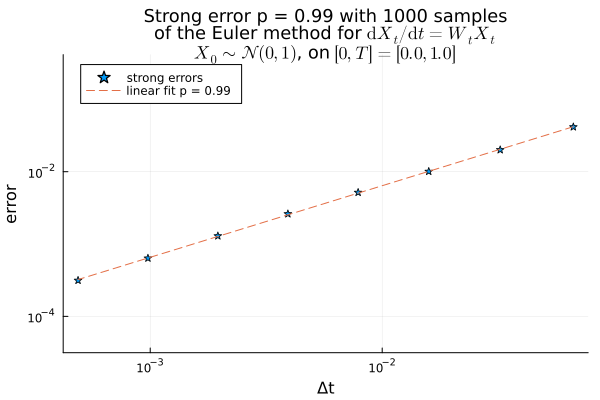
\includegraphics[scale=0.7]{img/order_linearhomogenous.png}
    \caption{Convergence of the strong error for the Euler approximation of $\mathrm{d}X_t/\mathrm{d}t = W_t X_t$, with initial condition $X_0 \sim \mathcal{N}(0, 1)$, on the time interval $[0, 1]$, based on 1000 sample paths, for each of the time steps in $\mathrm{d}t = 1/N$, with $N = 16, 32, 64, 128, 256, 512, 1024, 2048$.}
\end{figure}

\begin{rmk}
The extra multiplicative exponential term involving $\sum_i Z_i$ is estimated to be, since these random variables are independent, of order 
\begin{multline*}
    \mathbb{E}\left[\left|e^{\sum_i Z_i} - 1\right|\right] \sim \mathbb{E}\left[\left|\sum_i Z_i\right|\right] \leq \left(\mathbb{E}\left[\left(\sum_i Z_i\right)^2\right]\right)^{1/2} \\
    = \left(\sum_i \mathbb{E}\left[Z_i^2\right]\right)^{1/2} \sim \left(\sum_i \Delta t_N^3 \right)^{1/2} = \left(t_j \Delta t_N^2\right)^{1/2} \sim \Delta t_N
\end{multline*}
hence of strong order 1 in $\Delta t_N$. Therefore, this term does not affect the order of convergence of the Euler method, but it is of crucial importance when analysing higher order methods. In fact, the Heun method, which also seems to be of strong order 1, converges with strong order 2 to the average solution when given the noise at the mesh points, i.e.
\begin{equation}
    \label{barXtlinearhomogeneousrode}
    \bar X_t = X_0 e^{\sum_{i = 0}^{j-1}\left(\frac{1}{2}\left(W_{t_i} + W_{t_{i+1}}\right)(t_{i+1} - t_i) + (t_{i+1}-t_i)^3/24\right)},
\end{equation}
or to the approximation discarding this term altogether, i.e.
\begin{equation}
    \label{tildeXtlinearhomogeneousrode}
    \tilde X_t = X_0 e^{\sum_{i = 0}^{j-1}\left(\frac{1}{2}\left(W_{t_i} + W_{t_{i+1}}\right)(t_{i+1} - t_i)\right)},
\end{equation}
but it falls down to strong order 1 when the correct distribution \eqref{Xtlinearhomogeneousrode} for the exact solution is considered. This highlights the importance of using either the right distribution to check the order of convergence, or a higher order approximation. The focus of this article is on the Euler method, not Heun's, so we do not pursuit this point further. We limit ourselves to displaying the Figure \ref{figheunconvergence}, on which our observations above are based.
\end{rmk}

\begin{figure}[htb]
    \label{figheunconvergence}
    \caption{Order of convergence of the Heun method for the equation $\mathrm{d}X_t/\mathrm{d}t = W_t X_t$, with initial condition $X_0 \sim \mathcal{N}(0, 1)$, on the time interval $[0, 1]$, based on 1000 sample paths, for each of the time steps in $\mathrm{d}t = 1/N$, with $N = 16, 32, 64, 128, 256, 512, 1024$, towards sample paths of (i) exact solutions as in \eqref{Xtlinearhomogeneousrode}; (ii) average solutions as in \eqref{barXtlinearhomogeneousrode}; (iii) approximate solutions as in \eqref{barXtlinearhomogeneousrode}.}
\end{figure}

\subsection{Linear inhomogeneous equation}


We now consider the following linear equation with noise in the nonhomogenous term:
\begin{equation}
    \label{linearnonhomogeneousrode}
    \begin{cases}
        \displaystyle \frac{\mathrm{d}X_t}{\mathrm{d} t} = -X_t + W_t, \qquad 0 \leq t \leq T, \\
        \left. X_t \right|_{t = 0} = X_0,
      \end{cases}
\end{equation}
This has the explicit solution
\begin{equation}
    X_t = e^{-t}X_0 + \int_0^t e^{-(t-s)}W_s\;\mathrm{d}s.
\end{equation}

As in \cref{seclinearhomogeneousrode}, when we compute an approximate solution via Euler's method, we only draw the realizations $\{W_{t_i}\}_{i=0}^n$ of a sample path, on the mesh points. We can find the exact distribution for $\int_0^{t_j} e^{s} W_s\;\mathrm{d}s$ given the values of the noise at the mesh points and use that to draw feasible exact solutions to estimate the strong error.

First we break down the sum into parts:
\begin{equation}
    \int_0^{t_j} e^s W_s\;\mathrm{d}s = \sum_{i = 0}^{j-1} \int_{t_i}^{t_{i+1}} e^s W_s\;\mathrm{d}s.
\end{equation}
On each mesh interval $[t_i, t_{i+1}]$, we consider, again, the Brownian bridge
\begin{equation}
    B_t^i = W_t - W_{t_i} - \frac{t - t_i}{t_{i+1}-t_i}(W_{t_{i+1}} - W_{t_i}).
\end{equation}
Then,
\begin{align*}
    \int_{t_i}^{t_{i+1}} e^s W_s\;\mathrm{d}s & = \int_{t_i}^{t_{i+1}} e^s B_s^i\;\mathrm{d}s + \int_{t_i}^{t_{i+1}} e^s\left( W_{t_i} + \frac{s - t_i}{t_{i+1}-t_i}(W_{t_{i+1}} - W_{t_i})\right)\;\mathrm{d}s \\
    & = W_{t_{i+1}}e^{t_{i+1}} - W_{t_i}e^{t_i} - \frac{W_{t_{i+1}}-W_{t_i}}{t_{i+1}-t_i}\left(e^{t_{i+1}}-e^{t_i}\right) + Z_i,
\end{align*}
where
\begin{equation}
    Z_i = \int_{t_i}^{t_{i+1}} e^s B_s^i\;\mathrm{d}s.
\end{equation}
As before, the second term is a Gaussian with zero mean, and we need to compute its variance to completely characterize it. By translation, it suffices to consider a Brownian bridge $\{B_t\}_{t\in [0, \tau]}$ on an interval $[0, \tau]$, with $\tau = \Delta t_N$. This is obtained from $B_t = W_t - (t/\tau)W_\tau$. We have, since $\mathbb{E}[W_tW_s] = \min\{t, s\}$, that
\[
    \mathbb{E}[B_tB_s] = \min\{t, s\} - \frac{ts}{\tau}.
\]
Hence,
\begin{align*}
    \mathbb{E}\left[\left(\int_0^{\tau} e^s B_s\;\mathrm{d}s\right)^2\right] & = \mathbb{E}\left[\int_0^{\tau} \int_0^\tau e^s e^t B_sB_t\;\mathrm{d}s\;\mathrm{d}\right] \\
    & = \int_0^\tau \int_0^\tau e^s e^t \mathbb{E}[B_sB_t] \;\mathrm{d}s\;\mathrm{d}t \\
    & = \int_0^\tau \int_0^\tau e^s e^t\left(\min\{t, s\} - \frac{ts}{\tau}\right) \;\mathrm{d}s\;\mathrm{d}t \\
    & = \int_0^\tau \int_0^t e^s e^t s\;\mathrm{d}s\;\mathrm{d}t + \int_0^\tau \int_t^\tau e^s e^t t\;\mathrm{d}s\;\mathrm{d}t - \int_0^\tau \int_0^\tau e^s e^t \frac{ts}{\tau} \;\mathrm{d}s\;\mathrm{d}t \\
    & = \int_0^\tau e^t(te^t-e^t+1)\;\mathrm{d}t + \int_0^\tau te^t(e^\tau - e^t)\;\mathrm{d}t \\
    & \qquad - \int_0^\tau \frac{te^t}{\tau}\left(\tau e^\tau - e^\tau + 1\right)\;\mathrm{d}t \\
    & = \frac{\tau^3}{12}.
\end{align*}

Back to $Z_i$, this means that
\begin{equation}
    \label{linearnonhomogeneousZidistribution}
    Z_i \sim \mathcal{N}\left(0, \frac{(t_{i+1}- t_i)^3}{12}\right) = \frac{\sqrt{(t_{i+1} - t_i)^3}}{\sqrt{12}}\mathcal{N}(0, 1).
\end{equation}

For a normal variable $N \sim \mathcal{N}(\mu, \sigma)$, the expectation of the random variable $e^N$ is $\mathbb{E}[e^N] = e^{\mu + \sigma^2/2}$. Hence,
\begin{equation}
    \mathbb{E}[e^{Z_i}] = e^{((t_{i+1}- t_i)^3)/24}.
\end{equation}
This is the contribution of this random variable to the mean of the exact solution. But we actually need to use the exact $e^{\sum_i Z_i}$ for a more reliable estimate.

Hence, once an Euler approximation of \eqref{linearnonhomogeneousrode} is computed, along with realizations $\{W_{t_i}\}_{i=0}^n$ of a sample path of the noise, we consider an exact solution given by
\begin{equation}
    \label{Xtlinearnonhomogeneousrode}
    X_t = X_0 e^{\sum_{i = 0}^{j-1}\left(\frac{1}{2}\left(W_{t_i} + W_{t_{i+1}}\right)(t_{i+1} - t_i) + Z_i\right)},
\end{equation}
for realizations $Z_i$ drawn from a normal distributions given by \eqref{linearnonhomogeneousZidistribution}. Figure \ref{samplepathslinearnonhomogeneousrode} shows an approximate solution and a few sample paths of possible exact solutions associated with the given realizations of the noise on the mesh points.
\begin{figure}
    \label{samplepathslinearnonhomogeneousrode}
    \caption{Euler approximation of $\mathrm{d}X_t/\mathrm{d}t = W_t X_t$ with $X_0 = 1.0$, on $[0, T]$, and a few sample paths of exact solutios compatible with the given realizations of the noise on the mesh points.}
\end{figure}

The Table \ref{tablinearnonhomogeneousrode} shows the estimated strong error obtained from a thousand sample paths for each chosen time step, with initial condition $X_0 \sim \mathcal{N}(0, 1)$, on the interval $[0, T]$. The Figure \ref{figlinearnonhomogeneousrode} illustrates the order of convergence.

\begin{table}
    \label{tablinearnonhomogeneousrode}
    \begin{tabular}[htb]{l|l|l}
        1 & 2 & 3 \\
        4 & 5 & 6
    \end{tabular}
    \caption{blah}
\end{table}

\begin{figure}[htb]
    \label{figlinearnonhomogeneousrode}
    \caption{Convergence of the strong error for the Euler approximation of $\mathrm{d}X_t/\mathrm{d}t = W_t X_t$, with initial condition $X_0 \sim \mathcal{N}(0, 1)$, on the time interval $[0, 1]$, based on 1000 sample paths, for each of the time steps in $\mathrm{d}t = 1/N$, with $N = 16, 32, 64, 128, 256, 512, 1024$.}
\end{figure}

\subsection{Population dynamics with harvest}

Here, we consider a population dynamics modelled by a logistic equation (loosely inspired by \cite[Section 15.2]{HanKloeden2017}) with harvest:
\begin{equation}
    \label{rodepopulationdynamics}
    \frac{\mathrm{d}X_t}{\mathrm{d}t} = Z_t X_t (r - X_t) - H_t
\end{equation}
where $r > 0$ is constant, $\{Z_t\}_{t \geq 0}$ is a stochastic process playing the role of a random growth parameter, and $\{H_t\}_{t\geq 0}$ is a nonnegative point process playing the role of the harvest term. More specifically, $\{Z_t\}_{t \geq 0}$ is given by
\[
    Z_t = \lambda (1 + \varepsilon \sin(Y_t)),
\]
where $0 < \varepsilon < 1$ and $\{Y_t\}_{t\geq 0}$ is a geometric Brownian motion process, hence of the form \eqref{YtItonoise}-\eqref{Itonoiseterms}, and $\{H_t\}_{t\geq 0}$ is a point process of the form ...

We suppose the initial condition is non-negative and bounded almost surely:
\[
    0 \leq X_0 \leq R,
\]
for some $R > r$.

The noise process $\{Z_t\}_{t \geq 0}$ itself satisfies
\[
    0 < \lambda - \varepsilon \leq Z_t \leq \lambda + \varepsilon < 2\lambda, \qquad \forall t \geq 0.
\]

Define 
\[
    f(t, x, z) = z x(r - x)
\]
and notice that $f(t, x, z)x \geq 0$, for $x \geq 0$ and $z \geq 0$, and $f(t, x, z)x \leq 0$, for $x \geq r$ and $z \geq 0$. Hence the interval $[0, R]$ in $x$ is positively invariant and the pathwise solutions of \eqref{rodepopulationdynamics} are almost surely bounded as well, with
\[
    0 \leq X_t \leq R,
\]
for all $t \geq 0$.

The function $f=f(t, x, z)$ is continuously differentiable infinitely many times and with
\[
    \left|\frac{\partial f}{\partial x}(t, x, z)\right| = |z(r - 2x)|\leq 2\lambda (2R - r),
\]
for $|x| \leq R$ and $0 \leq z \leq 2\lambda$. In turn, the function $z = z(y) = \lambda (1 + \varepsilon \sin(y))$ is also continuously differentiable infinitely many times and is uniformly bounded along with all its derivatives.

The right hand side of \eqref{rodepopulationdynamics} is not globally Lipschitz, but, for the sake of analysis, since $X_t$ and $Y_t$ are bounded, the right hand side can be modified to a twice continuously differentiable, uniformly globally Lipschitz function $\tilde f(t, x, y)$ that coincides with $f(t, x, y)$ for $(t, x, y) \in \mathbb{R}\times [0, R]\times [0, 2\lambda]$ and satisfies \eqref{Lxassumptionbasic} with
\[
    L_X = 2\lambda (2R - r).
\]

Thus, the RODE \eqref{rodepopulationdynamics} with $0\leq X_0 \leq R$ almost surely, for some $R > r$, is equivalent to the RODE
\begin{equation}
    \label{rodepopulationdynamicstruncated}
    \frac{\mathrm{d}X_t}{\mathrm{d}t} = \tilde f(t, X_t, Y_t).
\end{equation}

With $\tilde f=\tilde f(t, x, y)$, the \cref{standinghypotheses1} hold. Moreover, it follows from \eqref{XtboundLXMt} (notice $M_t = 0$ here) that
\[
    |X_t| \leq |X_0|e^{2\lambda (2R - r)t} \leq R e^{2\lambda (2R - r)T}, \qquad 0 \leq t \leq T.
\]
almost surely. 

Therefore, all the conditions of \cref{thmItonoise} hold and the Euler method is of strong order 1.

\subsection{Earthquake and other impulse driven models}

See Neckel and Rupp pg 582 as a starting point of a model driven by a transport process as the source of ground motion excitation (both Kanai-Tajima and Bogdanoff, check out also the Clough-Penzien).

\appendix{}

\section{Discrete Gronwall Lemma}

We end this section by abstracting away the Gronwall type inequality we use \textcolor{red}{(this is probably written somewhere, and I need to find the source)}:
\begin{lem}
Let $(e_j)_j$ be a (finite or infinite) sequence of positive numbers satisfying
\begin{equation}
  \label{integralgronwall}
  e_j \leq a \sum_{i=0}^{j-1} e_i + b,
\end{equation}
with $e_0 = 0$, where $a, b > 0$. Then,
\begin{equation}
  \label{estimateintegralgronwall}
  e_j \leq b e^{aj}, \qquad \forall j.
\end{equation}
\end{lem}

\begin{proof}
  The result is trivially true for $j=0$. Suppose, by induction, that the result is true up to $j-1$. Then,
  $$
  e_j \leq a \sum_{i=0}^{j-1} be^{ai} + b = b \left(a \sum_{i=0}^{j-1} e^{ai} + 1\right).
  $$
  Using that $1 + a \leq e^a$, we have $a \leq e^a - 1$, hence
  $$
  e_j \leq b\left((e^a - 1)\sum_{i=0}^{j-1} e^{ia} + 1\right).
  $$
  Using that $\sum_{i=0}^{j-1} \theta^i = (\theta^j - 1)(\theta - 1)$, with $\theta = e^a$, we see that
  $$
  (e^a - 1)\sum_{i=0}^{j-1} e^{ia} \leq e^{ja} - 1,
  $$
  so that
  $$
  e_j \leq be^{ja},
  $$
  which completes the induction.
\end{proof}

\section{Numerical examples}

\subsection{Lower-order converge}

\begin{figure}
  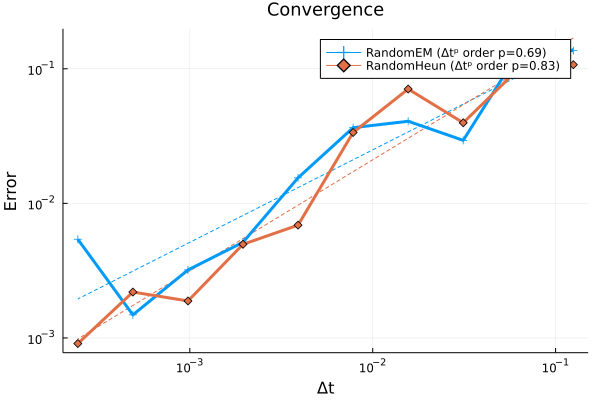
\includegraphics[scale=0.8]{img/plot_13.png}
\end{figure}

For a lower order convergence, below order $1$, we take the noise $\{Y_t\}_t$ to be the transport process defined by
$$
Y_t = \sin(t/Z)^{1/3},
$$
where $Z$ is a beta random variable $Z \sim B(\alpha, \beta)$. Notice $Z$ takes values strictly within $(0, 1)$ and, hence, $\sin(t/Z)$ can have arbitrarily high frequencies and, hence, go through the critic value $y = 0$ extremely often.

\textcolor{red}{(Need to remove the Heun method and do more tests and examples)}.

\section*{Acknowledgments}

\begin{thebibliography}{25}
    \bibitem{Asai2016} Y. Asai, \emph{Numerical Methods for Random Ordinary Differential Equations and their Appli-
    cations in Biology and Medicine.} Dissertation, Institut für Mathematik, Goethe Universität Frankfurt am Main, 2016.

    \bibitem{Bender2003} C. Bender, An It\^o formula for generalized functionals of a fractional Brownian motion with arbitrary Hurst parameter, \emph{Stochastic Processes and their Applications,} 104 (2003), 81--106.

    \bibitem{BHOB2008} F. Biagini, Y. Hu, B. Oksendal, T. Zhang. \emph{Stochastic Calculus for Fractional Brownian Motion and Applications,} Springer-Verlag, London, 2008.

    \bibitem{CoddingtonLevinson1985} E. A. Coddington, N. Levinson, \emph{Theory of Ordinary Differential Equations,} New York: McGraw-Hill, 1987.

    \bibitem{GruneKloeden2001} L. Gr\"une, P.E. Kloeden, Higher order numerical schemes for affinely controlled nonlinear systems, \emph{Numer. Math.} 89 (2001), 669--690.

    \bibitem{HanKloeden2017} X. Han \& P. E. Kloeden (2017), \emph{Random Ordinary Differential Equations and Their Numerical Solution,} Probability Theory and Stochastic Modelling, vol. 85, Springer Singapore. \href{https://link.springer.com/book/10.1007/978-981-10-6265-0}{DOI: 10.1007/978-981-10-6265-0}.

    \bibitem{Mishura2008} Y. S. Mishura2008, \emph{Stochastic calculus for fractional Brownian motion and related processes,} Lecture Notes in Mathematics 1929, Springer-Verlag, Berlin, Heidelberg, 2008.

\end{thebibliography}

\end{document}